%%%%%%%%%%%%%%%%%%%%%%%%%%%%%%%%%%%%%%%%%%%%%%%%%%%%%%%%%%%%%%%%%%%%%%
%%% PAGE SETUP
%%%%%%%%%%%%%%%%%%%%%%%%%%%%%%%%%%%%%%%%%%%%%%%%%%%%%%%%%%%%%%%%%%%%%%
\documentclass[11pt]{article}
\usepackage[a4paper,margin=3cm]{geometry}
\emergencystretch=1.5em

%%%%%%%%%%%%%%%%%%%%%%%%%%%%%%%%%%%%%%%%%%%%%%%%%%%%%%%%%%%%%%%%%%%%%%
%%% PACKAGE LIST
%%%%%%%%%%%%%%%%%%%%%%%%%%%%%%%%%%%%%%%%%%%%%%%%%%%%%%%%%%%%%%%%%%%%%%
\usepackage[T1]{fontenc}      % proper font encoding
\usepackage{lmodern}          % vector T1 fonts (else EC bitmaps)
\usepackage{amsmath}          % displays, flalign for calculational proofs
\usepackage{amssymb}          % blackboard bold, symbols
\usepackage{amsthm}           % theorem environments
\usepackage{mathtools}        % \coloneqq
\usepackage{tikz}             % figures (one fig_*.tex file each)
\usetikzlibrary{decorations.markings}
\usepackage{placeins}         % \FloatBarrier for Figures 4 and 5
\usepackage[hidelinks]{hyperref} % loaded last
\hypersetup{
  pdftitle={Mixed partition functions are exactly the graph
    parameters of exponentially bounded edge-connection rank},
  pdfauthor={William Whistler},
  pdfsubject={Graph parameters, connection matrices, and mixed
    partition functions},
  pdfkeywords={graph parameter, connection matrix, partition
    function, mixed partition function, edge-colouring model,
    symmetric tensor category, super vector space, fibre functor,
    Schur functor}}

%%%%%%%%%%%%%%%%%%%%%%%%%%%%%%%%%%%%%%%%%%%%%%%%%%%%%%%%%%%%%%%%%%%%%%
%%% THEOREM ENVIRONMENTS  (one counter, numbered by subsection;
%%% definitions and remarks live in prose, never in environments)
%%%%%%%%%%%%%%%%%%%%%%%%%%%%%%%%%%%%%%%%%%%%%%%%%%%%%%%%%%%%%%%%%%%%%%
\newtheorem{theo}{Theorem}[section]
\newtheorem{lemm}[theo]{Lemma}
\newtheorem{coro}[theo]{Corollary}
\newtheorem{obse}[theo]{Observation}

%%%%%%%%%%%%%%%%%%%%%%%%%%%%%%%%%%%%%%%%%%%%%%%%%%%%%%%%%%%%%%%%%%%%%%
%%% SHORTCUT LIST
%%%
%%% Notation ledger (one letter, one meaning, whole paper):
%%%   f      the graph parameter (pervasive; hence xi/eta below)
%%%   h      the Regts--Sevenster vertex functional
%%%   t      fragment arity (connection matrices M_{f,t})
%%%   tau_m  trace power sequence tr(g^m)  [draft's t_m renamed]
%%%   J      the parity-transfer involution  [draft's tau renamed]
%%%   \parityop  the parity operator on V   [draft's p renamed]
%%%   xi_i, eta_i  odd basis vectors        [RS21's f_i, g_i renamed:
%%%          f is reserved for graph parameters -- policing sentence
%%%          appears at the point of definition]
%%%   a', b' counts of alpha's/beta's in Appendix A [draft's p, q
%%%          renamed: p_h is RS notation]
%%%   u, v   generic morphisms in trace-calculus lemmas
%%%   g      generic endomorphism
%%%   z      zeta-function variable;  A  growth constant (appendix);
%%%   s      square size (appendix);  R  the rank bound;
%%%   k, 2l  even/odd colour counts (RS notation, kept)
%%%   F      fragments in ss2.2/3.1-3.2; Eulerian edge subsets in
%%%          ss2.4/5.4/6 (RS notation) -- the two uses never co-occur
%%%%%%%%%%%%%%%%%%%%%%%%%%%%%%%%%%%%%%%%%%%%%%%%%%%%%%%%%%%%%%%%%%%%%%
% --- graphs and fragments ---
\newcommand{\emptygraph}{\varnothing}
\newcommand{\freecircle}{\bigcirc}
\newcommand{\Frag}[1]{\mathfrak{F}_{#1}}          % t-fragments
\newcommand{\connmat}[2]{M_{#1,#2}}               % connection matrix
\newcommand{\glue}{\ast}                          % full gluing
\newcommand{\strand}{I}                           % the strand
\newcommand{\halfedges}[2]{\delta_{#1}(#2)}       % half-edges at #2 on edges of #1
% --- categories ---
\newcommand{\conncat}{\mathcal{C}_{f}}            % the connection category
\newcommand{\cauchy}{\mathcal{D}_{f}}             % its Cauchy completion
\newcommand{\unitobj}{\mathbf{1}}                 % monoidal unit
\newcommand{\genX}{X}                             % the generating object
\newcommand{\Kar}{\operatorname{Kar}}
\newcommand{\Add}{\operatorname{Add}}
\newcommand{\End}{\operatorname{End}}
\newcommand{\Hom}{\operatorname{Hom}}
\newcommand{\tr}{\operatorname{tr}}
\newcommand{\rk}{\operatorname{rk}}
% --- super linear algebra ---
\newcommand{\fib}{\omega}                         % the fibre functor
\newcommand{\svect}{\mathrm{sVect}_{\mathbb{C}}}
\newcommand{\str}{\operatorname{str}}
\newcommand{\parityop}{\mathfrak{p}}              % parity operator on V
\newcommand{\copair}{C}                           % the copairing
\newcommand{\twistedC}{\widehat{C}}               % the twisted element
\newcommand{\mate}[1]{#1^{\flat}}                 % the mate of a tensor
\newcommand{\symq}[1]{\varpi_{#1}}                % quotient to Sym^d
\newcommand{\SymV}{\operatorname{Sym}}
\newcommand{\parinv}{J}                           % parity-transfer involution
% --- appendix ---
\newcommand{\hook}[2]{H(#1,#2)}                   % the fat hook
\newcommand{\tzeta}[1]{\zeta_{#1}}                % trace zeta function
\newcommand{\Res}{\operatorname{Res}}

%%%%%%%%%%%%%%%%%%%%%%%%%%%%%%%%%%%%%%%%%%%%%%%%%%%%%%%%%%%%%%%%%%%%%%
%%% FRONT MATTER
%%%%%%%%%%%%%%%%%%%%%%%%%%%%%%%%%%%%%%%%%%%%%%%%%%%%%%%%%%%%%%%%%%%%%%
\title{Mixed partition functions are exactly the graph parameters of
exponentially bounded edge-connection rank}
\author{William Whistler\\
\texttt{will@whistler.uk}}
\date{}

\begin{document}
\maketitle

\begin{abstract}
We prove a conjecture of Regts and Sevenster: a complex-valued graph
parameter $f$ with $f(\emptygraph)=1$ has exponentially bounded
edge-connection rank if and only if it is a mixed partition function;
moreover, the model may be chosen with its numbers of even and odd
colours explicitly bounded in terms of the rank bound. From $f$ we
construct a connection category, a rigid symmetric
$\mathbb{C}$-linear monoidal category
whose morphism spaces have the connection ranks as dimensions and
whose trace pairings are nondegenerate. The rank hypothesis forces
moderate tensor growth, and a recent theorem of Etingof and Penneys
then shows that every nilpotent endomorphism has trace zero; together
with the nondegeneracy of the trace pairing, this makes the category
semisimple, and a theorem of Deligne provides a faithful symmetric
tensor functor to finite-dimensional super vector spaces. We then
identify the resulting super tensor network with the Regts--Sevenster
model exactly, viz.\ with its Eulerian-subgraph expansion and its sign
of $-1$ for every fermionic circuit. An appendix gives an independent and
direct proof of the nilpotent-trace step, showing that in a rigid
symmetric $\mathbb{C}$-linear category with
$\End(\unitobj)=\mathbb{C}$, exponentially
bounded endomorphism growth makes
the trace zeta function of every endomorphism rational, with explicit
degree bounds.

\medskip
\noindent\textit{MSC 2020:} 05C31, 18M05 (primary); 15A72, 05E05,
20C30 (secondary).

\noindent\textit{Keywords:} graph parameter; connection matrix;
partition function; mixed partition function; edge-colouring
model; symmetric tensor category; super vector space; fibre
functor; Schur functor.
\end{abstract}

\tableofcontents

%%%%%%%%%%%%%%%%%%%%%%%%%%%%%%%%%%%%%%%%%%%%%%%%%%%%%%%%%%%%%%%%%%%%%%
\section{Introduction}\label{sec:intro}
%%%%%%%%%%%%%%%%%%%%%%%%%%%%%%%%%%%%%%%%%%%%%%%%%%%%%%%%%%%%%%%%%%%%%%

Which graph parameters are partition functions? The question has
organised a substantial body of work since de la Harpe and Jones
\cite{dHJ93} introduced spin and vertex models on graphs as
generalisations of the models of statistical mechanics --- in
later terminology, vertex-colouring and edge-colouring models
respectively. Freedman,
Lov\'asz and Schrijver \cite{FLS07} characterised the partition
functions of vertex-colouring models by reflection positivity and
a rank condition on connection matrices; Szegedy \cite{Sze07} did
the same for edge-colouring models, with the complex case
characterised in \cite{DGLRS12}; and Schrijver characterised
the partition functions of spin models \cite{Sch13} and of
complex edge-colouring models \cite{Sch15} by rank growth.
The connection-matrix method is treated at length in Lov\'asz's
book \cite{Lov12}, and its categorical undercurrent --- that
connection matrices are Gram matrices of a category of fragments
--- goes back at least to Lov\'asz and Schrijver \cite{LS09}.

Regts and Sevenster \cite{RS21}, building on their symplectic
models \cite{RS17}, enlarged the edge-colouring world by a
fermionic sector: their \emph{mixed partition functions},
recalled in Section~\ref{subsec:mpf}, are partition functions of
edge-colouring models on a super vector space
$\mathbb{C}^{k|2\ell}$, and they include, for instance, every
evaluation of the characteristic polynomial
\cite[Prop.~10]{RS21}; the evaluation at zero, in particular, is
not the partition function of any ordinary edge-colouring model
\cite[Prop.~9]{RS21}. They proved that every mixed
partition function has exponentially bounded edge-connection rank
\cite[Thm~6]{RS21} and conjectured the converse. The history of
that conjecture calls for care: a 2017 extended abstract
announced the characterisation as a theorem
\cite[Thm~3.1]{RS17ea}, and
the full paper records that the announcement was mistaken --- the
orthosymplectic Lie superalgebra had incorrectly been claimed to
play no role --- and states the converse as a conjecture instead
\cite[abstract and footnotes~1--2]{RS21}, noting that the
expected proof route
through the invariant theory of the orthosymplectic supergroup
meets a serious obstruction, the non-reductivity of
$\mathfrak{osp}$; the completion of that route was deferred to a
companion manuscript which has, to our knowledge, not appeared.
A related
conjecture --- an algebraic characterisation of the mixed
partition functions of a fixed $\mathbb{C}^{k|2\ell}$ --- appears
as Conjecture~5.7 of Sevenster's thesis \cite{Sev18}.

This paper proves the conjecture. The slogan is that a purely
combinatorial exponential-rank condition forces a hidden
finite-dimensional super tensor model; the precise statement is
as follows.

\begin{theo}[Main Theorem]\label{theo:main}
A complex-valued graph parameter $f$, defined on finite multigraphs
with free circles permitted and normalised by $f(\emptygraph)=1$, has
exponentially bounded edge-connection rank if and only if it is a
mixed partition function. More precisely, if
$\rk \connmat{f}{t}\le R^{t}$ for some integer $R\ge 1$ and all
$t\ge 0$, then $f=p_{h}$ for a functional
$h\in(\SymV\mathbb{C}^{k}\otimes\Lambda\mathbb{C}^{2\ell})^{*}$
with $k,2\ell\le\lfloor 2eR\rfloor$, where $e$ is the base of the
natural logarithm.
\end{theo}

The implication from mixed partition functions to exponentially
bounded rank is Regts and Sevenster's theorem, with
$R=\max(1,k+2\ell)$; our contribution is the converse, together
with the dimension bound. Note that the hypothesis includes $t=0$, and
this is essential: multiplicativity of $f$ over disjoint unions
is not assumed but \emph{derived} from it
(Lemma~\ref{lemm:mult}), a small but pleasant surprise.

The proof runs as follows. From $f$ we construct a
\emph{connection category} $\conncat$: fragments modulo the
kernel of the connection pairing, organised into a rigid
symmetric monoidal category whose morphism spaces have the
connection ranks as their dimensions and whose trace pairings
are nondegenerate (Section~\ref{sec:conncat}). Its Cauchy
completion $\cauchy$ then satisfies the hypotheses of a recent
theorem of Etingof and Penneys \cite{EP26} --- the rank bound
becomes moderate tensor growth --- so every nilpotent
endomorphism has trace zero; combined with the nondegeneracy of
the trace pairing this makes $\cauchy$ semisimple abelian, and
Deligne's theorem \cite{Del02} provides an exact faithful
symmetric tensor functor to finite-dimensional super vector
spaces (Section~\ref{sec:semisimple}).

The remainder of the proof is the concrete half. The fibre
functor yields a form, a copairing and one vertex tensor per
degree, and $f$ becomes the value of a super tensor network
(Section~\ref{sec:extraction}). A separate reconstruction theorem
then identifies that network, after a parity normalisation, with
the Regts--Sevenster sum exactly --- Eulerian subgraphs,
orientations, pairings, and the sign of $-1$ for every fermionic
circuit (Section~\ref{sec:circuit}).

The categorical route never touches the invariant theory of
$\mathfrak{osp}$, which is how the non-reductivity obstruction
is bypassed.

Two of the ingredients deserve explicit billing. First, the
theorem of Etingof and Penneys, proved independently of the
present work and in much greater generality, is what carries the
semisimplicity step; Appendix~\ref{app:zeta} gives an
independent and direct proof of that step for our setting,
with a stronger conclusion --- in a rigid symmetric
$\mathbb{C}$-linear category with $\End(\unitobj)=\mathbb{C}$ and
exponentially bounded endomorphism growth, the trace zeta
function of \emph{every} endomorphism is rational, with explicit
degree bounds --- and it is this quantitative form that yields
the bound $k,2\ell\le\lfloor 2eR\rfloor$. Secondly, the
reconstruction theorem of
Section~\ref{sec:circuit} is where the conjecture-specific work
happens: Deligne's theorem produces an abstract fibre functor,
and turning that into the exact normalisations of
\cite[Definition~5]{RS21} is a sign-sensitive computation that
neither his theorem nor
\cite{EP26} performs. In adjacent work on the Holant framework,
Young \cite{You25} has proved a converse Holant theorem deriving
an orthogonal transformation from indistinguishability, and Cai
and Young \cite{CY26} analogous results through orbit closures
for the general linear group (see also \cite{CG22}); these concern
a different notion of equivalence and do not characterise by
rank growth.

The proof
gives the coarse bound $k,2\ell\le\lfloor 2eR\rfloor$ on the
colour dimensions,
but it provides no algorithm for constructing the functional $h$
and no effective bounds on its coordinates, Deligne's functor being
non-constructive; we do not pursue hypotheses weaker than a
uniform exponential connection-rank bound; and we work in
characteristic zero throughout.

Both implications of the Main Theorem, including the bound
$k,2\ell\le\lfloor 2eR\rfloor$, have been machine-checked in
Lean~4 over mathlib, with Deligne's theorem \cite[Thm~0.6]{Del02}
as the only axiomatised input \cite{Whi26};
Theorem~\ref{theo:zeta} is formalised in its stated generality,
and the nilpotent-trace step is carried by it, not by
\cite{EP26}. The formal development presents
the vertex functional in sorted colour order, in the sense of the
convention discussion of Section~\ref{subsec:paritytransfer}.

\subsection{Reading guide}\label{subsec:overview}

The sections follow the proof architecture above literally:
conventions and Definition~5 (\S\ref{sec:prelim}), the connection
category and its Cauchy completion (\S\ref{sec:conncat}),
semisimplicity and the fibre functor (\S\ref{sec:semisimple}),
extraction (\S\ref{sec:extraction}), reconstruction and the proof
of the Main Theorem (\S\ref{sec:circuit}), consequences
(\S\ref{sec:consequences}), and the independent proof of the
nilpotent-trace step (Appendix~\ref{app:zeta}). The
connection-category and reconstruction arguments are developed
self-containedly; beyond them the proof uses stated results of
Etingof--Penneys and of Deligne, and the standard representation
theory of symmetric groups.

%%%%%%%%%%%%%%%%%%%%%%%%%%%%%%%%%%%%%%%%%%%%%%%%%%%%%%%%%%%%%%%%%%%%%%
\section[Mixed partition functions, fragments, and half-edge
conventions]{Mixed partition functions, fragments, and half-edge
\mbox{conventions}}\label{sec:prelim}
%%%%%%%%%%%%%%%%%%%%%%%%%%%%%%%%%%%%%%%%%%%%%%%%%%%%%%%%%%%%%%%%%%%%%%

The purpose of this section is twofold: to fix our conventions for
multigraphs, fragments and gluing, and to state the Regts--Sevenster
definition of a mixed partition function together with the hypothesis
class of the Main Theorem.

\subsection{Graphs, half-edges, and parameters}\label{subsec:graphs}

A \emph{graph} is a finite multigraph: loops, parallel edges, and
\emph{free circles} --- closed edges incident with no vertex,
isomorphic to the circle $\freecircle$ --- are all permitted. We write
$\emptygraph$ for the empty graph and $G\sqcup H$ for disjoint union.
A \emph{graph parameter} is a function from isomorphism classes of
graphs to $\mathbb{C}$. We write $\mathbb{N}=\mathbb{Z}_{\ge0}$.

Every edge other than a free circle consists of two \emph{half-edges},
one at each endpoint; the two half-edges of a loop are distinct and
lie at the same vertex. The degree $\deg(v)$ counts half-edges, so
that a loop contributes two, and for $F\subseteq E$ we write
$\halfedges{F}{v}$ for the set of half-edges at $v$ belonging to edges
of $F$. Throughout this paper, orders, orientations and pairings of edges
are carried by the half-edges, while colours are assigned to edges
and inherited by both half-edges; this convention does real work at
loops and parallel edges, and we shall rely on it without further
comment. A fully formal
treatment would encode a graph by a finite
vertex set, a finite half-edge set, an incidence map, a perfect
matching of half-edges into edges, and a nonnegative integer
recording the free-circle components, which carry no half-edges;
we shall not need this formal encoding explicitly.

\subsection{Fragments and gluing}\label{subsec:fragments}

Intuitively, a fragment is a graph with some dangling edge-ends, which
may later be glued to the dangling ends of another fragment.
Formally, a \emph{$t$-fragment} is a graph together with exactly $t$
distinguished vertices of degree one, labelled $1,\dotsc,t$; the edge
at the $i$-th labelled vertex is the \emph{open end} $i$. We write
$\Frag{t}$ for the set of isomorphism classes of $t$-fragments, so
that $\Frag{0}$ is the set of graphs. To \emph{glue} two open ends,
delete the two labelled vertices and unify their edges into a single
edge; for $F,G\in\Frag{t}$, the \emph{full gluing}
$F\glue G\in\Frag{0}$ glues the $i$-th open end of $F$ to the $i$-th
open end of $G$ for every $i$. Note that gluing two open ends whose
edges have both endpoints labelled produces a free circle; this is
the reason free circles are admitted from the outset. We show two
examples, including this degenerate case, in
Figure~\ref{fig:gluing}.

\begin{figure}
\centering
% fig_gluing.tex -- gluing two fragments, incl. the free-circle case.
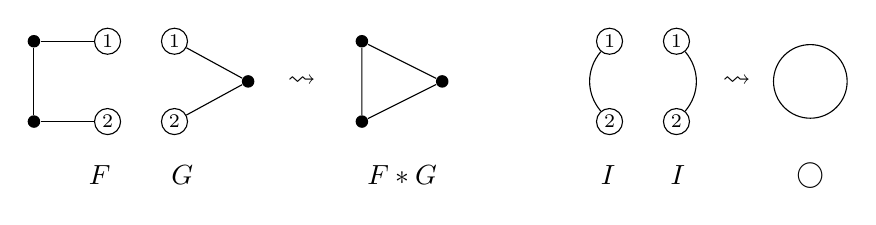
\begin{tikzpicture}[scale=0.85,
  vert/.style={circle,fill,inner sep=1.6pt},
  lab/.style={circle,draw,inner sep=1.2pt,font=\scriptsize}]
  % (a) two 2-fragments glued into a closed graph
  \begin{scope}
    \node[vert] (a) at (0,0.6) {};
    \node[vert] (b) at (0,-0.6) {};
    \draw (a) -- (b);
    \node[lab] (l1) at (1.1,0.6) {1};
    \node[lab] (l2) at (1.1,-0.6) {2};
    \draw (a) -- (l1); \draw (b) -- (l2);
    \node[lab] (m1) at (2.1,0.6) {1};
    \node[lab] (m2) at (2.1,-0.6) {2};
    \node[vert] (c) at (3.2,0) {};
    \draw (m1) -- (c); \draw (m2) -- (c);
    \node at (1.6,-1.4) {$F$\hspace{2.2em}$G$};
    \node at (4.0,0) {$\leadsto$};
    \node[vert] (a2) at (4.9,0.6) {};
    \node[vert] (b2) at (4.9,-0.6) {};
    \node[vert] (c2) at (6.1,0) {};
    \draw (a2) -- (b2); \draw (a2) -- (c2); \draw (b2) -- (c2);
    \node at (5.5,-1.4) {$F\glue G$};
  \end{scope}
  % (b) degenerate case: strand glued to strand gives a free circle
  \begin{scope}[xshift=8.6cm]
    \node[lab] (p1) at (0,0.6) {1};
    \node[lab] (p2) at (0,-0.6) {2};
    \draw (p1) to[bend right=40] (p2);
    \node[lab] (q1) at (1.0,0.6) {1};
    \node[lab] (q2) at (1.0,-0.6) {2};
    \draw (q1) to[bend left=40] (q2);
    \node at (0.5,-1.4) {$\strand\qquad\strand$};
    \node at (1.9,0) {$\leadsto$};
    \draw (3.0,0) circle (0.55);
    \node at (3.0,-1.4) {$\freecircle$};
  \end{scope}
\end{tikzpicture}

\caption{Gluing two fragments; the free-circle-creating case.}
\label{fig:gluing}
\end{figure}

Two further operations on fragments, composition and the identity
strand, are introduced at the start of Section~\ref{sec:conncat},
where their elementary properties are established.

\subsection{Connection matrices and the hypothesis
class}\label{subsec:connmat}

The \emph{edge-connection matrix} $\connmat{f}{t}$ of a graph
parameter $f$ is the $\Frag{t}\times\Frag{t}$ matrix with entries
\[
\connmat{f}{t}(F,G)\coloneqq f(F\glue G),
\]
and its rank $\rk\connmat{f}{t}$ is the supremum of the ranks of its
finite submatrices. The hypotheses of the Main Theorem are:
\begin{itemize}
\item[(H1)] $f(\emptygraph)=1$;
\item[(H2)] there is an integer $R\ge 1$ with
  $\rk\connmat{f}{t}\le R^{t}$ for all $t\ge 0$.
\end{itemize}
A real bound $r$ may be replaced by $\lceil r\rceil$, so the
integrality of $R$ costs no generality. Note that $t=0$ is included
in (H2); this is essential, and is the source of the automatic
multiplicativity of $f$ (Lemma~\ref{lemm:mult}).

\subsection{Mixed partition functions}\label{subsec:mpf}

The definition of a mixed partition function recalled in this
subsection is Definition~5 of \cite{RS21}, and we cite it by that
number, theirs, throughout the paper.

Fix $k,\ell\in\mathbb{N}$ and let $V=V_{0}\oplus V_{1}$ be a super
vector space with $\dim V_{0}=k$ and $\dim V_{1}=2\ell$, with
distinguished bases $e_{1},\dotsc,e_{k}$ of $V_{0}$ and
$\xi_{1},\dotsc,\xi_{2\ell}$ of $V_{1}$. To avoid confusion we write
$\xi_{i},\eta_{i}$ where \cite{RS21} write $f_{i},g_{i}$, reserving
the letter $f$ for graph parameters throughout this paper; here
\[
\eta_{i}\coloneqq
\begin{cases}
-\xi_{i+\ell}& i\le \ell,\\
\hphantom{-}\xi_{i-\ell}& i>\ell,
\end{cases}
\]
so that each $\eta_{i}$ is a signed basis vector. Let
$h\in(\SymV V_{0}\otimes\Lambda V_{1})^{*}$. Regts and Sevenster
permit an arbitrary such functional; since the exterior degree
appearing at a vertex in the sum below is $\deg_{F}(v)$, which is
even whenever $F$ is Eulerian, the odd exterior part of $h$ never
contributes, and we may therefore impose, without loss of
generality, that $h$ vanishes on every component of odd exterior
degree.

Call $F\subseteq E(G)$ \emph{Eulerian} if $\deg_{F}(v)$ is even for
every vertex $v$. For Eulerian $F$, choose an Eulerian orientation
of $F$ together with a compatible \emph{local pairing}
$\kappa=(\kappa_{v})_{v}$, which pairs at each vertex $v$ each
incoming half-edge of $\halfedges{F}{v}$ with an outgoing one; we
list each pair as $(a_{1},a_{2})$ with $a_{1}$ incoming. Following
the pairs from edge to edge decomposes $F$ into directed
\emph{$\kappa$-circuits}, and we write $c(\kappa)$ for their
number. The
\emph{mixed partition function} of $h$ is the graph parameter
\begin{multline*}
p_{h}(G)\coloneqq
\sum_{\substack{F\subseteq E(G)\\ F\text{ Eulerian}}}
(-1)^{c(\kappa)}
\sum_{\psi\colon E\setminus F\to[k]}\;
\sum_{\varphi\colon F\to[2\ell]}\\
\prod_{v\in V(G)}
h\Bigl(
\bigodot_{a\in\halfedges{E\setminus F}{v}}\hspace{-1ex}e_{\psi(a)}
\;\otimes
\bigwedge_{(a_{1},a_{2})\in\kappa_{v}}\hspace{-1ex}
\xi_{\varphi(a_{1})}\wedge\eta_{\varphi(a_{2})}
\Bigr),
\end{multline*}
for a graph $G$ without free circles, extended to all graphs by
$p_{h}(\freecircle)\coloneqq k-2\ell$ and multiplicativity over
disjoint union. Here $\psi$ and $\varphi$ colour edges, and each
half-edge inherits the colour of its edge. The wedge over the
pairs of $\kappa_{v}$ is unambiguous: each factor
$\xi_{\varphi(a_{1})}\wedge\eta_{\varphi(a_{2})}$ has even
exterior degree, so the order of the pairs is immaterial and the
displayed argument of $h$ is a well-defined element of
$\SymV V_{0}\otimes\Lambda V_{1}$. The value is independent
of the choice of orientation and compatible local pairing:
\cite[Proposition~3]{RS21} proves this for the skew sector, and
the mixed sum reduces to it, one colouring $\psi$ at a time, in
the discussion preceding their Definition~5. A graph parameter is a \emph{mixed
partition function} if it equals $p_{h}$ for some $k$, $\ell$ and
$h$ as above.

Regts and Sevenster proved that every mixed partition function
satisfies (H2), with $R=\max(1,k+2\ell)$
\cite[Theorem~6]{RS21} --- the maximum matters only for the
degenerate model with $k=2\ell=0$ --- and (H1) is immediate, the
empty graph carrying the empty product; the Main Theorem is the
converse.

The definition is somewhat intricate, and so we now give an
explicit example, to which we shall return. Take $k=2$ and
$\ell=1$, fix $\theta\in\mathbb{C}$, and let
$h=h(\theta)$ be determined by
\[
h(e_{1}^{\odot i})=\theta,\qquad
h(e_{1}^{\odot i}\odot e_{2})=\sqrt{-1},\qquad
h(e_{1}^{\odot i}\otimes \xi_{1}\wedge\eta_{1})=1
\qquad(i\ge 0),
\]
and by $h=0$ on all basis elements outside the span of these. Regts
and Sevenster showed \cite[Proposition~10]{RS21} that, for graphs
without free-circle components, $p_{h(\theta)}$ is the
characteristic polynomial $G\mapsto\det(\theta I-A_{G})$, where
the adjacency matrix $A_{G}$ counts a loop twice on the diagonal;
since $k-2\ell=0$ here, $p_{h(\theta)}$ vanishes on every graph
that does contain a free circle.

We evaluate $p_{h(\theta)}$ on the graph $L$ with one vertex and one
loop; see Figure~\ref{fig:definitionfive}. The loop has two
half-edges at the single vertex $v$, so $\deg(v)=2$, and both
$F=\emptyset$ and $F=\{\text{loop}\}$ are Eulerian. For
$F=\emptyset$, the vertex factor is
$h(e_{\psi}\odot e_{\psi})$: the colouring $\psi=1$ contributes
$h(e_{1}^{\odot 2})=\theta$, while $\psi=2$ contributes
$h(e_{2}^{\odot 2})=0$. For $F=\{\text{loop}\}$, the pairing
$\kappa_{v}$ joins the loop's two half-edges into a single
$\kappa$-circuit, so $c(\kappa)=1$; the
colouring $\varphi=j$ contributes $h(\xi_{j}\wedge\eta_{j})$, and
since
\[
\xi_{1}\wedge\eta_{1}
=-\xi_{1}\wedge\xi_{2}
=\xi_{2}\wedge\eta_{2},
\]
both odd colours contribute through the same basis vector of
$\Lambda^{2}V_{1}$, each with value $1$. In total
\[
p_{h(\theta)}(L)
=\theta+(-1)^{1}\cdot(1+1)
=\theta-2
=\det\bigl(\theta I-A_{L}\bigr),
\]
as required, since $A_{L}=(2)$. It is worth pausing on what this
small computation has already exercised: the two incidences of a
loop, the Eulerian condition, the circuit sign, the
distinction between a loop and a free circle, and the fact that the
$\eta$-convention makes distinct odd colourings contribute through a
common basis vector. All five phenomena return in earnest in
Sections~\ref{sec:extraction} and~\ref{sec:circuit}.

\begin{figure}
\centering
% fig_definitionfive.tex -- the loop graph L, its two Eulerian
% subsets, the pairing kappa at the vertex.
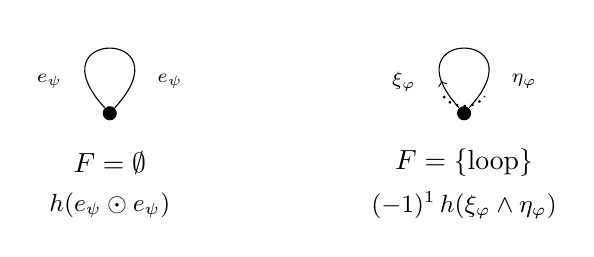
\begin{tikzpicture}[scale=0.9,
  vert/.style={circle,fill,inner sep=1.8pt}]
  % left pane: F = empty, both half-edges carry even colours
  \begin{scope}
    \node[vert] (v) at (0,0) {};
    \draw (v) .. controls (-1.1,1.2) and (1.1,1.2) .. (v);
    \node[font=\scriptsize] at (-0.85,0.45) {$e_{\psi}$};
    \node[font=\scriptsize] at (0.85,0.45) {$e_{\psi}$};
    \node at (0,-0.7) {$F=\emptyset$};
    \node[font=\small] at (0,-1.3) {$h(e_{\psi}\odot e_{\psi})$};
  \end{scope}
  % right pane: F = {loop}, oriented; kappa pairs the two half-edges
  \begin{scope}[xshift=5cm]
    \node[vert] (w) at (0,0) {};
    \draw[postaction={decorate},decoration={markings,
      mark=at position 0.2 with {\arrow{>}}}]
      (w) .. controls (-1.1,1.2) and (1.1,1.2) .. (w);
    \node[font=\scriptsize] at (-0.85,0.45) {$\xi_{\varphi}$};
    \node[font=\scriptsize] at (0.85,0.45) {$\eta_{\varphi}$};
    \draw[dotted,thick] (-0.29,0.24) to[bend right=55] (0.29,0.24);
    \node at (0,-0.7) {$F=\{\text{loop}\}$};
    \node[font=\small] at (0,-1.3)
      {$(-1)^{1}\,h(\xi_{\varphi}\wedge\eta_{\varphi})$};
  \end{scope}
\end{tikzpicture}

\caption{The loop graph $L$, its two Eulerian subsets, and the
pairing $\kappa$.}
\label{fig:definitionfive}
\end{figure}

%%%%%%%%%%%%%%%%%%%%%%%%%%%%%%%%%%%%%%%%%%%%%%%%%%%%%%%%%%%%%%%%%%%%%%
\section{The connection category and its Cauchy
completion}\label{sec:conncat}
%%%%%%%%%%%%%%%%%%%%%%%%%%%%%%%%%%%%%%%%%%%%%%%%%%%%%%%%%%%%%%%%%%%%%%

We now organise fragments and gluing into a symmetric monoidal
category $\conncat$, whose morphism spaces have the connection ranks
as their dimensions, and complete it to a category $\cauchy$ in which
the remainder of the proof takes place. The category theory involved is elementary and self-contained:
every trace identity below is proved by exhibiting an equality of
glued graphs, and $f$ is applied only afterwards. For readers of a
combinatorial bent, the following dictionary may serve as a guide.

\begin{center}
\begin{tabular}{ll}
number of open ends & object\\
fragment & morphism\\
gluing & composition\\
disjoint union & tensor product\\
full closure & trace\\
connection pairing & trace pairing
\end{tabular}
\end{center}

We call $\conncat$ the \emph{connection category} of $f$. To avoid
confusion we do not use the term skein category, which is established
in quantum topology for a related but distinct circle of ideas.

\subsection{Composition of fragments}\label{subsec:composition}

Fragments compose by partial gluing, and we fix the categorical
order once and for all: a fragment $F\in\Frag{s+t}$ is read as a
morphism from its first $s$ open ends (its \emph{inputs}) to its
last $t$ (its \emph{outputs}), and for $F\in\Frag{s+t}$ and
$G\in\Frag{t+u}$ the \emph{composite} $G\circ F\in\Frag{s+u}$ ---
first $F$, then $G$, written right to left --- glues the last $t$
open ends of $F$ to the first $t$ open ends of $G$, in order. The
inputs of $G\circ F$ are the inputs of $F$ with their labels, and
its outputs are the outputs of $G$, relabelled
$s+1,\dotsc,s+u$. The \emph{strand}
$\strand\in\Frag{2}$ is the fragment with a single edge joining its
two labelled vertices, and more generally, for a permutation $\pi$ of
$[t]$, the \emph{permutation fragment} $P_{\pi}\in\Frag{t+t}$
consists of $t$ disjoint strands joining open end $i$ to open end
$t+\pi(i)$. Whenever a disjoint union of fragments is read as a
morphism, it carries the input--input--output--output block
relabelling made explicit in Section~\ref{subsec:categorydef}.

\begin{lemm}\label{lemm:gluingfacts}
The following hold for all fragments of compatible arities.
\begin{enumerate}
\item[(i)] Composition is associative:
  $(H\circ G)\circ F=H\circ(G\circ F)$.
\item[(ii)] The strand is an identity: writing $\strand^{t}$ for
  $t$ disjoint strands, $F\circ\strand^{s}=F=\strand^{u}\circ F$ for
  $F\in\Frag{s+u}$.
\item[(iii)] Composition and disjoint union interchange: for
  $F\in\Frag{s+t}$, $G\in\Frag{t+u}$, $F'\in\Frag{s'+t'}$ and
  $G'\in\Frag{t'+u'}$,
  $(G\sqcup G')\circ(F\sqcup F')=(G\circ F)\sqcup(G'\circ F')$.
\item[(iv)] Gluing commutes with simultaneous relabelling of the
  interface, and $P_{\pi}\circ P_{\sigma}=P_{\pi\sigma}$, where
  $\pi\sigma$ denotes the composite function ($\sigma$ first).
\end{enumerate}
\end{lemm}

\begin{proof}
All four statements are instances of one description of iterated
gluing. A gluing is the quotient of the edge multiset of a disjoint
union along a pairing of open ends: each matched pair of pendant
edges is unified into one edge, chains of matched strands collapse
into single edges, and closed chains collapse into free circles. In
an iterated composite each open end participates in at most one
interface pair, so the union of the interface pairings is itself a
single pairing on ends, and unifying iteratively in any order equals
unifying simultaneously along that union; this proves (i). For (ii),
gluing a strand's end to an open end $o$ of $F$ deletes the two
labelled vertices and unifies the strand's edge with the edge of
$o$, yielding a single pendant edge ending at the strand's other
labelled vertex, which is $F$ with that open end relabelled. For
(iii), the interface pairing of the left-hand side splits as the
disjoint union of the blockwise pairings, and quotienting a disjoint
union along a split pairing is the disjoint union of the quotients.
Finally (iv): a relabelling is an isomorphism of the data the
pairing is defined on, and composing permutation fragments
concatenates strands, which by (ii) collapse to the strands of the
composite permutation.
\end{proof}

\subsection{The connection category}\label{subsec:categorydef}

For the remainder of the paper, $f$ denotes a graph parameter
satisfying (H1) and (H2) with rank bound $R$. We begin with a small
surprise: multiplicativity of $f$ need not be assumed, because the
$t=0$ case of (H2) provides it.

\begin{lemm}\label{lemm:mult}
For all graphs $G$ and $H$ we have $f(G\sqcup H)=f(G)f(H)$.
\end{lemm}

\begin{proof}
At $t=0$, hypothesis (H2) reads $\rk\connmat{f}{0}\le R^{0}=1$, and
$\connmat{f}{0}(G,H)=f(G\sqcup H)$. The row of $\emptygraph$ is
$(f(H))_{H}$, which is nonzero since $f(\emptygraph)=1$ by (H1).
A matrix of rank at most one with a nonzero row has every row a
scalar multiple of it: $f(G\sqcup H)=c_{G}f(H)$ for some
$c_{G}\in\mathbb{C}$, and setting $H=\emptygraph$ gives
$c_{G}=f(G)$.
\end{proof}

Let $\mathbb{C}^{(\Frag{t})}$ denote the vector space of finite
formal $\mathbb{C}$-combinations of $t$-fragments, and let
\[
\Theta_{t}\colon\mathbb{C}^{(\Frag{t})}\to
\bigl(\mathbb{C}^{(\Frag{t})}\bigr)^{*},
\qquad
\Theta_{t}(F)\coloneqq\bigl(G\mapsto f(F\glue G)\bigr),
\]
extended linearly, with kernel
$N_{t}\coloneqq\ker\Theta_{t}$. The quotient
$\mathbb{C}^{(\Frag{t})}/N_{t}$ has dimension exactly
$\rk\connmat{f}{t}$: it is isomorphic to the image of $\Theta_{t}$,
i.e.\ to the row space of the connection matrix, and any finite
linearly independent family of rows remains independent after
restriction to a suitable finite set of columns, so the row-space
dimension equals the supremum of the finite-submatrix ranks. By
(H2) this dimension is at most $R^{t}$; this is how the rank
hypothesis will enter every dimension count below.

\begin{lemm}\label{lemm:ideal}
The kernels $N$ form an ideal for both operations, in the following
sense.
\begin{enumerate}
\item[(a)] If $x\in N_{s+t}$ and $w$, $y$ are fragments of
  compatible arities, then $w\circ x\circ y\in N$.
\item[(b)] If $x\in N_{s+t}$ and $z\in\Frag{s'+t'}$, then
  $x\sqcup z\in N_{(s+s')+(t+t')}$.
\end{enumerate}
\end{lemm}

\begin{proof}
For (a), any full closure of $w\circ x\circ y$ against a fragment
$G$ performs, by Lemma~\ref{lemm:gluingfacts}(i), the same
simultaneous unification as the full closure of $x$ against
$y\circ G\circ w$; since $x\in N$, the value of $f$ on the latter
vanishes for every $G$. For (b), given a closure $G$ of
$x\sqcup z$, first glue the open ends of $z$ into $G$, obtaining a
fragment $G_{z}$ of arity $s+t$, possibly with extra closed
components; then
$f\bigl((x\sqcup z)\glue G\bigr)=f(x\glue G_{z})=0$.
\end{proof}

We may now define the category. The \emph{connection category}
$\conncat$ has objects the natural numbers, the object $t$ being
written $\genX^{\otimes t}$; its morphism spaces are
\[
\Hom(\genX^{\otimes s},\genX^{\otimes t})
\coloneqq\mathbb{C}^{(\Frag{s+t})}/N_{s+t},
\]
a fragment being read as a morphism from its first $s$ open ends to
its last $t$; composition is induced by the composition of
fragments, which descends to the quotients by
Lemma~\ref{lemm:ideal}(a), and the identity of $\genX^{\otimes t}$
is the class of $\strand^{t}$, by Lemma~\ref{lemm:gluingfacts}(ii).
The tensor product is addition on objects and is induced by
disjoint union on morphisms, with the block relabelling that the
input--output reading demands: for $F\in\Frag{s+t}$ and
$F'\in\Frag{s'+t'}$, the disjoint union is read as a morphism with
inputs the inputs of $F$ followed by those of $F'$ and outputs the
outputs of $F$ followed by those of $F'$; concretely, $F$-input
$i\mapsto i$, $F'$-input $i\mapsto s+i$, $F$-output
$j\mapsto s+s'+j$, and $F'$-output $j\mapsto s+s'+t+j$. This
descends by Lemma~\ref{lemm:ideal}(b); it is
strictly associative and unital with unit
$\unitobj\coloneqq\genX^{\otimes 0}$, since disjoint union of
isomorphism classes is so. Thus $\conncat$ is a
$\mathbb{C}$-linear strict monoidal category.

\begin{lemm}\label{lemm:simpleunit}
$\End(\unitobj)=\mathbb{C}\cdot[\emptygraph]$.
\end{lemm}

\begin{proof}
By construction
$\dim\End(\unitobj)=\rk\connmat{f}{0}$, which is $1$ by (H1) and
(H2), and $[\emptygraph]\ne 0$ since
$f(\emptygraph\glue\emptygraph)=1$.
\end{proof}

We henceforth identify $\End(\unitobj)$ with $\mathbb{C}$ via
$[\emptygraph]\mapsto 1$; every closed graph $G$ thereby represents
the scalar $f(G)$. Indeed $[G]=f(G)[\emptygraph]$: for every
closed graph $H$,
$f\bigl((G-f(G)\,\emptygraph)\sqcup H\bigr)
=f(G\sqcup H)-f(G)f(H)=0$ by Lemma~\ref{lemm:mult}, so
$G-f(G)\,\emptygraph\in N_{0}$.

The category is symmetric. The braiding of $\genX$ with itself is
the class of $P_{(1\,2)}$, and more generally the classes of the
permutation fragments realise every permutation of tensor factors;
by Lemma~\ref{lemm:gluingfacts}(iv) they compose as the permutations
do. Since the monoidal structure is strict, the hexagon axioms
reduce to identities among permutation fragments of the form
$P_{\pi\sqcup\mathrm{id}}\circ P_{\mathrm{id}\sqcup\pi}$, which hold
by the same composition rule; naturality of the braiding is
Lemma~\ref{lemm:gluingfacts}(iv) applied to the relabelling the
braiding performs; and the braiding squares to the identity.

The object $\genX$ is self-dual. Both the coevaluation
$\mathrm{coev}\in\Hom(\unitobj,\genX^{\otimes2})$ and the evaluation
$\mathrm{ev}\in\Hom(\genX^{\otimes2},\unitobj)$ are the class of the
strand $\strand$, read with both open ends as outputs and both as
inputs respectively; the snake identities are literal strand
unifications, viz.\ instances of Lemma~\ref{lemm:gluingfacts}(ii).
Consequently every object of $\conncat$ is self-dual: the
evaluation and coevaluation of $\genX^{\otimes t}$ are the classes
of $t$ parallel strands, the $i$-th end of one block joined to the
$i$-th end of the other, and the snake identities again reduce to
strand unifications. The \emph{trace} of
$u\in\End(\genX^{\otimes t})$ is its full strand closure --- the
scalar obtained by gluing the $i$-th output back to the $i$-th
input for every $i$. Every trace is thus an $f$-value of a closed
graph. In particular
\[
\tr(\mathrm{id}_{\genX})=f(\freecircle),
\]
the categorical dimension of $\genX$: closing a single strand
produces the free circle, which is the reason free circles were
admitted in Section~\ref{subsec:graphs}.

Finally, closed graphs decompose into stars. Let
$\sigma_{d}\in\Hom(\unitobj,\genX^{\otimes d})$ denote the class of
the \emph{$d$-star}: a single vertex with $d$ pendant edges, its
open ends labelled $1,\dotsc,d$; in particular $\sigma_{0}$ is
the isolated vertex. For a closed graph $G$ without free
circles, fix orders on its vertices and edges, and for each edge
an order of its two half-edges; then in $\conncat$
\begin{equation}\label{eq:stars}
[G]=
\Bigl(\bigotimes_{e\in E}\mathrm{ev}\Bigr)
\circ P_{G}\circ
\Bigl(\bigotimes_{v\in V}\sigma_{\deg v}\Bigr),
\end{equation}
where $P_{G}$ is the permutation fragment matching each star leg to
its half-edge. Indeed, the right-hand side glues the stars' pendant
edges in pairs along $E$, by
Lemma~\ref{lemm:gluingfacts}(i) and (iii), and each matched pair
unifies into the single edge $e$, reconstructing $G$; a loop sends
two legs of the same star to one evaluation, which is where the
half-edge convention of Section~\ref{subsec:graphs} earns its keep.

\subsection{The trace calculus}\label{subsec:tracecalc}

The following identities are standard consequences of rigidity and
symmetry, but in $\conncat$ they admit direct combinatorial proofs:
each asserts that two closed graphs are equal, and $f$ is applied
only afterwards. We prove them in this form because
Section~\ref{sec:semisimple} will lean on them before any further
structure is available. We abbreviate $uv\coloneqq u\circ v$.

\begin{lemm}\label{lemm:tracecalc}
Let $u$ and $v$ be morphisms of $\conncat$ of appropriate types.
\begin{enumerate}
\item[(a)] $\tr(uv)=\tr(vu)$ for
  $u\colon Y\to Z$ and $v\colon Z\to Y$.
\item[(b)] $\tr_{Y\otimes Z}(u\otimes v)=\tr(u)\tr(v)$ for
  $u\in\End(Y)$, $v\in\End(Z)$.
\item[(c)] $\tr\bigl(c_{Z,Z}\circ(u\otimes v)\bigr)=\tr(uv)$ for
  $u,v\in\End(Z)$, where $c$ is the braiding.
\end{enumerate}
\end{lemm}

\begin{proof}
(a) Both traces are the $f$-value of the same closed graph: the
strand closure of $u\circ v$ glues every open end of $u$ to the
matching open end of $v$ --- the composition interface directly, and
the outer legs through the closing strands, which merge away by
Lemma~\ref{lemm:gluingfacts}(ii) --- and the closure of $v\circ u$
performs the identical set of end-pairings.
(b) The closure of a disjoint union is the disjoint union of the
closures, and $f$ is multiplicative by Lemma~\ref{lemm:mult}.
(c) Closing $c\circ(u\otimes v)$ connects the output of $u$ through
the swap to the input of $v$, and the output of $v$ back to the
input of $u$; the resulting closed graph is the cyclic gluing of $u$
and $v$, which is exactly the closure of $u\circ v$, the
interface strands again merging away.
\end{proof}

\begin{lemm}\label{lemm:negligible}
If $u\in\Hom(\genX^{\otimes s},\genX^{\otimes t})$ satisfies
$\tr(uv)=0$ for every
$v\in\Hom(\genX^{\otimes t},\genX^{\otimes s})$, then $u=0$.
\end{lemm}

\begin{proof}
The trace closure of $u$ against a fragment $v$ differs from the
defining pairing $u\glue G$ of Section~\ref{subsec:categorydef} only
by a fixed relabelling of the $s+t$ open ends. Relabelling is a
bijection on fragments, so the two families of test values coincide,
and the hypothesis places a lift of $u$ in $N_{s+t}$.
\end{proof}

In the language of tensor categories, Lemma~\ref{lemm:negligible}
says that $\conncat$ has no nonzero negligible morphisms; it is the
single point at which the definition of $\conncat$ as a quotient
\emph{by} the connection kernel pays off, and it is the
engine of semisimplicity in Section~\ref{sec:semisimple}.

\subsection{The Cauchy completion}\label{subsec:cauchy}

The category $\conncat$ has neither direct sums nor images of
idempotents, and both will be needed. We therefore pass to the
\emph{Cauchy completion}
\[
\cauchy\coloneqq\Kar\bigl(\Add(\conncat)\bigr),
\]
where $\Add$ is the additive envelope --- objects are finite tuples
of objects of $\conncat$, morphisms are matrices --- and $\Kar$ is
the Karoubi envelope --- objects are pairs $(Y,e)$ with
$e\in\End(Y)$ idempotent, and morphisms $(Y,e)\to(Z,e')$ are the
$a\colon Y\to Z$ with $a=e'ae$. The Karoubi envelope of an additive
category is additive, with $(Y,e)\oplus(Z,e')=(Y\oplus Z,e\oplus
e')$, so $\cauchy$ admits finite direct sums and split idempotents
together.\footnote{The order matters: applying $\Add$ \emph{after}
$\Kar$ need not produce an idempotent-complete category, since a
summand of a direct sum need not be a direct sum of summands. The
distinction disappears once $\cauchy$ is known to be semisimple
(Section~\ref{sec:semisimple}), after which
$\Add(\Kar(\conncat))\simeq\cauchy$.}

The structure of $\conncat$ extends. The tensor product extends
bilinearly to tuples and to idempotent pairs, with the symmetry
acting componentwise; morphism spaces remain finite-dimensional,
being submatrices of matrices of morphism spaces of $\conncat$;
$\End(\unitobj)=\mathbb{C}$ persists, since $\mathbb{C}$ has no
nontrivial idempotents; and duals extend by
$(Y_{1},\dotsc,Y_{m})^{\vee}=(Y_{1}^{\vee},\dotsc,Y_{m}^{\vee})$
and $(Y,e)^{\vee}=(Y^{\vee},e^{\vee})$, with evaluation and
coevaluation corrected by the idempotents --- the cup is
$(e\otimes e^{\vee})\circ\mathrm{coev}_{Y}$ and the cap
$\mathrm{ev}_{Y}\circ(e^{\vee}\otimes e)$; the first snake
identity for $(Y,e)$ then unwinds to the defining formula of the
dual morphism $e^{\vee}$, and the second collapses onto the snake for
$Y$, so no new computation arises, and on tuples the snakes
reduce entrywise. Traces are computed accordingly:
the trace of a matrix of endomorphisms is the sum of the traces of
its diagonal entries, and the trace of $a\in\End(Y,e)$ is
$\tr_{Y}(a)$. Thus $\cauchy$ is a rigid symmetric
$\mathbb{C}$-linear monoidal category with finite-dimensional
morphism spaces and $\End(\unitobj)=\mathbb{C}$, and it is
generated by $\genX$
under tensor products, direct sums and summands.

The nondegeneracy of Lemma~\ref{lemm:negligible} survives the
completion; this small lemma is what will kill the Jacobson radical
in Section~\ref{sec:semisimple}, so we record it with care.

\begin{lemm}\label{lemm:nondegD}
Let $P$ and $Q$ be objects of $\cauchy$ and let $a\colon P\to Q$
satisfy $\tr(ba)=0$ for every $b\colon Q\to P$. Then $a=0$.
\end{lemm}

\begin{proof}
First let $P$ and $Q$ be objects of $\Add(\conncat)$, say with
components $(Y_{i})_{i}$ and $(Z_{j})_{j}$, and let
$a=(a_{ji})$ as a matrix. For fixed indices $i$ and $j$, let $b$
be the matrix supported in entry $(i,j)$ with value an arbitrary
$b_{ij}\colon Z_{j}\to Y_{i}$. Then
$\tr(ba)=\tr(b_{ij}a_{ji})=0$ for every $b_{ij}$, and
Lemma~\ref{lemm:negligible} gives $a_{ji}=0$; as $i$ and $j$ were
arbitrary, $a=0$.

Now let $P=(Y,e)$ and $Q=(Z,e')$ be objects of $\cauchy$ and
$a=e'ae\colon P\to Q$ with $\tr(ba)=0$ for all $b\colon Q\to P$.
For an arbitrary $c\colon Z\to Y$ in $\Add(\conncat)$, put
$b\coloneqq ece'$, a morphism $Q\to P$. Then, using $a=e'ae$ and
Lemma~\ref{lemm:tracecalc}(a),
\[
\tr(ca)=\tr(c\,e'ae)=\tr(ece'\,a)=\tr(ba)=0 ,
\]
and the first paragraph gives $a=0$.
\end{proof}

%%%%%%%%%%%%%%%%%%%%%%%%%%%%%%%%%%%%%%%%%%%%%%%%%%%%%%%%%%%%%%%%%%%%%%
\section{Moderate growth, nilpotent traces, and the super fibre
functor}\label{sec:semisimple}
%%%%%%%%%%%%%%%%%%%%%%%%%%%%%%%%%%%%%%%%%%%%%%%%%%%%%%%%%%%%%%%%%%%%%%

We are now ready to prove that $\cauchy$ is semisimple abelian
and admits a super fibre functor. The whole
argument rests on three facts: every object of $\cauchy$ has
moderate tensor growth; nilpotent endomorphisms have trace zero;
and the trace pairing is nondegenerate
(Lemma~\ref{lemm:nondegD}). The rest is finite-dimensional algebra
and a theorem of Deligne. Semisimplicity is \emph{not} automatic
for rigid symmetric categories --- without a growth hypothesis
there exist such categories containing nilpotent endomorphisms of
nonzero trace (see \cite[\S3.4]{EP26} for examples) --- and this
is precisely why the present section has content.

\subsection{Moderate growth and nilpotent traces}
\label{subsec:growth}

\begin{lemm}\label{lemm:growthD}
Let $Z\in\cauchy$ be a direct summand of
$\bigoplus_{j=1}^{m}\genX^{\otimes n_{j}}$ with $m\ge1$, and put
$n_{\max}\coloneqq\max_{j}n_{j}$. Then
\[
\dim\End(Z^{\otimes N})\le m^{2N}R^{2n_{\max}N}
\qquad(N\ge 0).
\]
In particular $\dim\End(Z^{\otimes N})<N!$ for all sufficiently
large $N$. Since every object of $\cauchy$ is such a summand, every
object of $\cauchy$ has moderate growth in the sense of
\cite{EP26}.
\end{lemm}

\begin{proof}
Put $Y\coloneqq\bigoplus_{j=1}^{m}\genX^{\otimes n_{j}}$ and
choose $\iota\colon Z\to Y$ and $\rho\colon Y\to Z$ with
$\rho\iota=\mathrm{id}_{Z}$. Tensoring this retraction shows that
$Z^{\otimes N}$ is a retract of $Y^{\otimes N}$, and
$g\mapsto\iota^{\otimes N}g\rho^{\otimes N}$ embeds
$\End(Z^{\otimes N})$ linearly into $\End(Y^{\otimes N})$, with
left inverse $a\mapsto\rho^{\otimes N}a\iota^{\otimes N}$. The
$N$-th tensor power of the sum expands into $m^{N}$ summands
$\genX^{\otimes|w|}$ indexed by words $w$, each with
$|w|\le n_{\max}N$, so
\[
\dim\End(Z^{\otimes N})
\le\sum_{w,w'}\dim\Hom\bigl(\genX^{\otimes|w|},
\genX^{\otimes|w'|}\bigr)
\le m^{2N}\,R^{2n_{\max}N},
\]
using (H2) for each summand. The right-hand side is exponential in
$N$, hence eventually smaller than $N!$.
\end{proof}

\begin{lemm}\label{lemm:qtrace}
The quantum trace of \cite{EP26} on $\cauchy$ coincides with the
closure trace of Section~\ref{subsec:tracecalc}.
\end{lemm}

\begin{proof}
Etingof and Penneys construct their quantum trace from the
Drinfeld isomorphism \cite[\S2.3]{EP26}. In a symmetric rigid
category, for $u\in\End(Y)$, that construction reduces to the
composite
\[
\unitobj
\xrightarrow{\ \mathrm{coev}_{Y}\ }
Y\otimes Y^{\vee}
\xrightarrow{\ u\otimes\mathrm{id}\ }
Y\otimes Y^{\vee}
\xrightarrow{\ c_{Y,Y^{\vee}}\ }
Y^{\vee}\otimes Y
\xrightarrow{\ \mathrm{ev}_{Y}\ }
\unitobj .
\]
In $\conncat$ the structural morphisms $\mathrm{coev}_{Y}$,
$c_{Y,Y^{\vee}}$ and $\mathrm{ev}_{Y}$ are represented by strand
and permutation fragments, and inserting $u$ into their composite
performs exactly the end-pairings of the full strand closure of
$u$, by Lemma~\ref{lemm:gluingfacts}. The identification extends
additively to $\Add(\conncat)$, and for a Karoubi object $(Y,e)$
it restricts to the idempotent summand: a morphism $a=eae$ has
trace $\tr_{Y}(a)$ on both sides.
\end{proof}

We shall apply the following theorem, extracted from
Corollary~1.5 of \cite{EP26} --- which gives the vanishing for
non-negligible indecomposable objects --- together with their
Lemma~1.6, which extends it to every object of a rigid category.

\begin{theo}[{Etingof--Penneys \cite[Cor.~1.5,
Lem.~1.6]{EP26}}]\label{theo:EP}
Let $\mathcal{B}$ be a Cauchy complete $\mathbb{C}$-linear braided
monoidal category with finite-dimensional morphism spaces and
$\End(\unitobj)=\mathbb{C}$, which is rigid and in which every
object has moderate growth. Then the quantum trace of every
nilpotent endomorphism in $\mathcal{B}$ is zero.
\end{theo}

\begin{theo}\label{theo:niltrace}
Every nilpotent endomorphism in $\cauchy$ has trace zero.
\end{theo}

\begin{proof}
The category $\cauchy$ satisfies every hypothesis of
Theorem~\ref{theo:EP}: it is Cauchy complete by construction
(Section~\ref{subsec:cauchy}); it is $\mathbb{C}$-linear and
symmetric, hence braided; its morphism spaces are
finite-dimensional; $\End(\unitobj)=\mathbb{C}$
(Lemma~\ref{lemm:simpleunit}); it is rigid; and every object has
moderate growth (Lemma~\ref{lemm:growthD}). By
Lemma~\ref{lemm:qtrace} the quantum trace is our trace.\footnote{%
Corollary~1.8 of \cite{EP26} packages the remainder of this
section's argument through semisimplification; we prefer the route
below because it exposes the role of the connection pairing.}
\end{proof}

Appendix~\ref{app:zeta} proves Theorem~\ref{theo:niltrace}
independently of \cite{EP26}: apply Theorem~\ref{theo:zeta} with
$A=m^{2}R^{2n_{\max}}$.

\subsection{Semisimplicity}\label{subsec:semisimplicity}

\begin{theo}\label{theo:radical}
For every $Y\in\cauchy$ the algebra $\End(Y)$ is semisimple.
\end{theo}

\begin{proof}
Let $j$ be an element of the Jacobson radical of the
finite-dimensional algebra $\End(Y)$ and let $u\in\End(Y)$ be
arbitrary. Then $ju$ lies in the radical, hence is nilpotent ---
the radical of a finite-dimensional algebra is a nilpotent ideal
--- so $\tr(ju)=0$ by Theorem~\ref{theo:niltrace}, and by cyclicity
(Lemma~\ref{lemm:tracecalc}(a)) also $\tr(uj)=0$. Now
Lemma~\ref{lemm:nondegD} applied with $a=j$ gives $j=0$.
\end{proof}

Decompose the identity of any $Y\in\cauchy$ into orthogonal
primitive idempotents of the semisimple algebra $\End(Y)$; since
idempotents split in $\cauchy$, this expresses $Y$ as a finite
direct sum of objects with primitive identity. We call an object
$S$ with $\End(S)=\mathbb{C}$ an \emph{atom} --- the word
\emph{simple} is reserved until the abelian structure is
available --- and the summands just
produced are atoms, because a corner $e\End(Y)e$ of a semisimple
$\mathbb{C}$-algebra at a primitive idempotent is a
finite-dimensional division algebra over the algebraically closed
field $\mathbb{C}$, hence $\mathbb{C}$ itself.

\begin{lemm}\label{lemm:dichotomy}
A nonzero morphism between atoms is an isomorphism, and
non-isomorphic atoms admit no nonzero morphisms between them.
\end{lemm}

\begin{proof}
Let $a\colon S\to T$ be nonzero with $S$, $T$ atoms. By
Lemma~\ref{lemm:nondegD} there is $b\colon T\to S$ with
$\tr(ba)\ne0$. Since $\End(S)=\mathbb{C}$ we have
$ba=\mu\,\mathrm{id}_{S}$ with $\mu\ne0$, so
$v\coloneqq\mu^{-1}b$ satisfies $va=\mathrm{id}_{S}$; then
$av\in\End(T)=\mathbb{C}$ is an idempotent, nonzero because
$ava=a\ne0$, hence $av=\mathrm{id}_{T}$. Thus $a$ is an
isomorphism.
\end{proof}

\begin{theo}\label{theo:semisimple}
Choose representatives $\{S_{\gamma}\}$ of the isomorphism classes
of atoms. The functor
$Y\mapsto\bigl(\Hom(S_{\gamma},Y)\bigr)_{\gamma}$ is an
equivalence of $\mathbb{C}$-linear categories between $\cauchy$
and the category of finite-support families of finite-dimensional
vector spaces. Consequently $\cauchy$ is semisimple abelian, its
tensor product is exact in each variable, and its simple objects
are the atoms.
\end{theo}

\begin{proof}
Every object is a finite direct sum of atoms, as shown above. By
Lemma~\ref{lemm:dichotomy}, for $Y\cong\bigoplus S_{\gamma(i)}$
and $Z\cong\bigoplus S_{\delta(j)}$ every morphism is a matrix
over the spaces
$\Hom(S_{\gamma},S_{\delta})=\delta_{\gamma\delta}\cdot\mathbb{C}$,
so the functor is fully faithful; a finite-support family
$(W_{\gamma})$ is the image of
$\bigoplus_{\gamma}S_{\gamma}^{\oplus\dim W_{\gamma}}$, so it is
essentially surjective. The target category is semisimple abelian,
and abelianness transports along the equivalence. Exactness of the
tensor product holds because in a semisimple abelian category
every short exact sequence splits and additive functors preserve
split exactness.
\end{proof}

\subsection{The super fibre functor}\label{subsec:fibrefunctor}

We may now verify the hypotheses of Deligne's theorem for
$\cauchy$:
\begin{itemize}
\item essentially small: the fragments form a set of
  representatives, and all Hom-spaces, idempotents, tuples and
  pairs built from them are set-sized;
\item abelian, $\mathbb{C}$-linear and semisimple, with
  finite-dimensional morphism spaces and with
  $\End(\unitobj)=\mathbb{C}$: Theorem~\ref{theo:semisimple} and
  Section~\ref{subsec:cauchy};
\item rigid and symmetric, with exact tensor product:
  Section~\ref{subsec:cauchy} and
  Theorem~\ref{theo:semisimple};
\item finitely tensor-generated by the self-dual object $\genX$:
  every object of $\cauchy$ is a direct summand of a finite
  direct sum of tensor powers of $\genX$; summands are subobjects
  in the semisimple abelian structure, and $\genX$ is self-dual,
  so this is tensor generation in Deligne's sense;
\item every object of moderate growth: in a semisimple category
  the length of $Y^{\otimes N}$ is at most
  $\dim\End(Y^{\otimes N})$ --- if
  $Y^{\otimes N}\cong\bigoplus_{i}S_{i}^{\oplus m_{i}}$ then the
  length is $\sum_{i}m_{i}\le\sum_{i}m_{i}^{2}=\dim\End$ --- and
  the latter is exponentially bounded by
  Lemma~\ref{lemm:growthD}.
\end{itemize}
In this list the
nilpotent-trace theorem enters only through
Theorem~\ref{theo:semisimple} --- the semisimple abelian
structure, together with the tensor exactness and the subobject
language that ride on it --- and everything else follows from
the rank bound and the constructions of
Section~\ref{sec:conncat} alone. The representation-theoretic
input thus enters the route to the fibre functor at exactly one
point.

\begin{theo}[{Deligne \cite[Thm~0.6]{Del02}; see also
\cite{Ost04}}]\label{theo:fibre}
There is an exact faithful $\mathbb{C}$-linear symmetric monoidal
functor $\fib\colon\cauchy\to\svect$.
\end{theo}

The remainder of the proof consumes less than the theorem
provides: only the existence of a symmetric monoidal
$\mathbb{C}$-linear functor to $\svect$ is used below --- the
nondegeneracy of $b$, the evenness and invariance of the vertex
tensors, and the transfer of the square's death are all carried
by functoriality alone, and the exactness and faithfulness of
$\fib$ play no further role.

Here the morphisms of $\svect$ are the parity-preserving linear
maps; we use this convention repeatedly. We fix such an $\fib$ once
and for all, suppress its structural isomorphisms
$\fib(Y)\otimes\fib(Z)\cong\fib(Y\otimes Z)$ from the notation
throughout, and write $V\coloneqq\fib(\genX)$, a super vector
space
$V=V_{0}\oplus V_{1}$ with $\dim V_{0}=k$ and, as we shall see in
Section~\ref{sec:extraction}, $\dim V_{1}=2\ell$ even.

The growth hypothesis also bounds the dimensions of $V$; this is
the source of the quantitative clause of the Main Theorem. We
borrow from Appendix~\ref{app:zeta} exactly one statement, whose
elementary symmetric-group proof is independent of everything in
this section. Here $\Phi_{n}$ denotes the symmetric-braiding
action of $\mathbb{C}[S_{n}]$ on the $n$-th tensor power, and
$e_{\lambda}$ the central idempotent of the block of
$\lambda\vdash n$.

\begin{lemm}[Square death; proved in
Appendix~\ref{app:zeta}]\label{lemm:squareimport}
Let $Z$ be an object of a rigid symmetric $\mathbb{C}$-linear
monoidal category with $\End(\unitobj)=\mathbb{C}$, satisfying
$\dim\End(Z^{\otimes n})\le A^{n}$ for all $n$ and some constant
$A\ge1$, and let $s$ be an integer with $s>2e\sqrt{A}$. Then
$\Phi_{s^{2}}(e_{(s^{s})})=0$ in $\End(Z^{\otimes s^{2}})$.
\end{lemm}

\begin{proof}
This is Lemma~\ref{lemm:squaredeath}, whose proof combines the
block-injection estimate of Lemma~\ref{lemm:blockdeath} with a
hook-length bound.
\end{proof}

\begin{coro}\label{coro:dimbound}
The dimensions of $V$ satisfy $k\le\lfloor 2eR\rfloor$ and
$\dim V_{1}\le\lfloor 2eR\rfloor$.
\end{coro}

\begin{proof}
Apply Lemma~\ref{lemm:squareimport} to $Z=\genX$ in $\cauchy$,
with growth constant $A=R^{2}$ by (H2): any integer $s>2eR$ ---
in particular the least one, $s=\lfloor 2eR\rfloor+1$ --- has
$\Phi_{s^{2}}(e_{(s^{s})})=0$ in $\End(\genX^{\otimes s^{2}})$.
Here, for $\lambda\vdash n$, choose a primitive idempotent
$q_{\lambda}$ in the
$\lambda$-block of $\mathbb{C}[S_{n}]$ and define
$S_{\lambda}(\genX)\coloneqq\operatorname{im}\Phi_{n}(q_{\lambda})$,
an image that exists because idempotents split in $\cauchy$. The
block being $\mathrm{Mat}_{d_{\lambda}}(\mathbb{C})$, the image
of its central identity $e_{\lambda}$ is a direct sum of
$d_{\lambda}$ isomorphic copies of $S_{\lambda}(\genX)$; so
$\Phi_{s^{2}}(e_{(s^{s})})$ projects onto the $(s^{s})$-isotypic
summand $S_{(s^{s})}(\genX)^{\oplus d_{(s^{s})}}$ of
$\genX^{\otimes s^{2}}$, and its vanishing is
equivalent to $S_{(s^{s})}(\genX)=0$ in $\cauchy$. Applying the
$\mathbb{C}$-linear symmetric monoidal functor $\fib$ carries
$\Phi_{s^{2}}(e_{(s^{s})})$ to the corresponding idempotent for
the super-permutation action on $V^{\otimes s^{2}}$, so
$S_{(s^{s})}(V)=0$ in $\svect$. By the hook criterion for super
vector spaces \cite[Cor.~1.9]{Del02} (in substance the theorem of
Berele and Regev \cite{BR87}), $S_{\lambda}(V)\ne0$ exactly when
$\lambda$ lies in the fat hook $\hook{\dim V_{0}}{\dim V_{1}}$,
where $\hook{a}{b}\coloneqq\{\lambda:\lambda_{a+1}\le b\}$
(Appendix~\ref{app:zeta});
the square $(s^{s})$ lies outside a fat hook $\hook{a}{b}$
precisely when $s>a$ and $s>b$. Hence $\dim V_{0}<s$ and
$\dim V_{1}<s$, i.e.\ both are at most $\lfloor 2eR\rfloor$. Note that the square is its own conjugate
partition, so the conclusion is insensitive to the row/column
convention in the hook criterion.
\end{proof}

%%%%%%%%%%%%%%%%%%%%%%%%%%%%%%%%%%%%%%%%%%%%%%%%%%%%%%%%%%%%%%%%%%%%%%
\section{From categorical tensors to a super tensor
network}\label{sec:extraction}
%%%%%%%%%%%%%%%%%%%%%%%%%%%%%%%%%%%%%%%%%%%%%%%%%%%%%%%%%%%%%%%%%%%%%%

In this section we extract from the fibre functor the raw data
of a mixed model --- a bilinear form, a copairing, and one vertex
tensor per degree --- and express $f$ as the value of a super tensor
network built from them. This section and the next are where
signs can go wrong; each sign below is paid exactly once, in a
numbered statement. The data map is
\[
\mathrm{ev}\mapsto b,\qquad
\mathrm{coev}\mapsto\copair,\qquad
\sigma_{d}\mapsto T_{d}\rightsquigarrow h^{\mathrm{cat}}_{d},\qquad
(\copair,h^{\mathrm{cat}})\rightsquigarrow
(\twistedC,h^{\mathrm{RS}})
\rightsquigarrow\text{Definition~5},
\]
and the subsections follow it: the form and its coordinates
(\S\ref{subsec:formcoords}), the copairing and its twist
(\S\ref{subsec:copairing}), the vertex tensors and the passage to
a tensor network (\S\ref{subsec:mates}), the change of
normalisation (\S\ref{subsec:paritytransfer}); the identification
with Definition~5 is then the business of
Section~\ref{sec:circuit}.

\subsection{The form and its coordinates}\label{subsec:formcoords}

Write $b\coloneqq\fib(\mathrm{ev})\colon V\otimes V\to\mathbb{C}$.
The form $b$ is even, since $\fib$ preserves the grading;
supersymmetric, since $\mathrm{ev}\circ c=\mathrm{ev}$ holds
already in $\conncat$ (gluing the swap into a strand yields a
strand); and nondegenerate, since the snake identities make
$x\mapsto b(x,-)$ invertible with inverse built from
$\fib(\mathrm{coev})$. The restriction of $b$ to $V_{1}$ is then a
nondegenerate antisymmetric form, so $\dim V_{1}$ is even; we
write $\dim V_{1}=2\ell$, and Corollary~\ref{coro:dimbound} bounds
both $k=\dim V_{0}$ and $2\ell$ by $\lfloor 2eR\rfloor$. Choose
coordinates
adapted to $b$: a basis $e_{1},\dotsc,e_{k}$ of $V_{0}$ with
$b(e_{i},e_{j})=\delta_{ij}$ and $b(e_{i},V_{1})=0$, and a basis
$\xi_{1},\dotsc,\xi_{2\ell}$ of $V_{1}$ with
\[
b(\xi_{m},\xi_{m+\ell})=1=-b(\xi_{m+\ell},\xi_{m})
\quad(m\le\ell),
\qquad
b(\xi_{i},\xi_{j})=0\ \text{otherwise}.
\]
With $\eta_{i}$ as in Section~\ref{subsec:mpf}, this gives
$b(\xi_{i},\eta_{i})=-1$ and $b(\eta_{i},\xi_{j})=\delta_{ij}$
for all $i,j$; the latter identity is verified entry by entry in
Lemma~\ref{lemm:twistedmaps} below.

For homogeneous $v_{i},w_{i}\in V$ define the
\emph{tensor-power pairing}
\[
\beta_{d}(v_{1}\otimes\dotsb\otimes v_{d},\,
w_{1}\otimes\dotsb\otimes w_{d})
\coloneqq
(-1)^{\sum_{i<j}|v_{j}||w_{i}|}\prod_{i=1}^{d}b(v_{i},w_{i}).
\]

\begin{lemm}\label{lemm:koszul}
For a fixed word of parities, the Koszul sign of a rearrangement
in $\svect$ equals the sign of the permutation it induces on the
odd letters; in particular the sign is multiplicative under
composition, and signed evaluations along any two rearrangement
paths realising the same permutation of the labelled homogeneous
tensor factors are equal. Consequently:
\begin{enumerate}
\item[(a)] $\beta_{d}$ is the signed evaluation obtained by
  rearranging $(v_{1}\dotsm v_{d}\,w_{1}\dotsm w_{d})$ into the
  interleaved word $(v_{1}w_{1}\,v_{2}w_{2}\dotsm v_{d}w_{d})$
  and applying $b$ to each adjacent pair;
\item[(b)] $\beta_{d}(\pi v,\pi w)=\beta_{d}(v,w)$ for the super
  $S_{d}$-action applied to both arguments.
\end{enumerate}
\end{lemm}

\begin{proof}
The symmetry of $\svect$ on homogeneous vectors is the flip times
$(-1)^{|x||y|}$, so a composite of symmetries multiplies the
scalars $(-1)$ once for each transposition of two odd letters;
this is precisely the sign of the induced permutation of the odd
letters, which is multiplicative, and any two decompositions
realising the same permutation of the labelled homogeneous
tensor factors agree by coherence of the symmetric structure. For (a), moving each $w_{i}$ leftward past
$v_{i+1},\dotsc,v_{d}$ costs exactly
$(-1)^{\sum_{i<j}|v_{j}||w_{i}|}$ on the support of the product of
the $b(v_{i},w_{i})$. For (b), each factor $b(v_{i},w_{i})$
forces $|v_{i}|=|w_{i}|$ on the support, so every interleaved
block $(v_{i}w_{i})$ has even total parity; acting by $\pi$ on
both arguments permutes these even blocks, which costs no sign,
and merely reindexes the scalar factors. Terms outside the
support vanish on both sides.
\end{proof}

\subsection{The copairing and the twisted
element}\label{subsec:copairing}

Write $\copair\coloneqq\fib(\mathrm{coev})\in V\otimes V$, and for
$D\in V\otimes V$ define $L_{D}\colon V\to V$ by
$L_{D}(x)\coloneqq(\mathrm{id}\otimes b)(D\otimes x)$, with no
reordering, so that $L_{D}(x)=\sum_{i}u_{i}\,b(w_{i},x)$ for
$D=\sum_{i}u_{i}\otimes w_{i}$. Applying $\fib$ to the snake
identity, which holds strictly in $\conncat$ by strand
unification, gives $L_{\copair}=\mathrm{id}_{V}$; and since $b$ is
nondegenerate, $L_{D}=L_{D'}$ forces $D=D'$, so this property
determines $\copair$ uniquely. In the coordinates above,
\[
\copair=\copair_{0}+\copair_{1},
\qquad
\copair_{0}=\sum_{i=1}^{k}e_{i}\otimes e_{i},
\qquad
\copair_{1}=\sum_{i=1}^{2\ell}\xi_{i}\otimes\eta_{i},
\]
as follows from the verification $L_{\copair_{0}+\copair_{1}}
=\mathrm{id}$ in Lemma~\ref{lemm:twistedmaps}.

Let $\parityop\colon V\to V$ denote the parity operator, and
define the \emph{twisted element}
\[
\twistedC\coloneqq(\parityop\otimes\mathrm{id})\copair
=\copair_{0}-\copair_{1},
\qquad\text{so that}\qquad
L_{\twistedC}=\parityop .
\]
The twisted element is not a copairing, and free circles must
never be evaluated through it. Indeed
\[
b(\copair)=k-2\ell=\operatorname{sdim}V,
\qquad
b(\twistedC)=k+2\ell=\str(\parityop),
\]
and the two values differ whenever $\ell>0$. Free circles are
carried by multiplicativity and by
$f(\freecircle)=\tr(\mathrm{id}_{\genX})
=\str(\mathrm{id}_{V})=k-2\ell$, the middle equality because a
symmetric monoidal functor takes categorical traces to
supertraces; they are removed \emph{before} the parity transfer of
Lemma~\ref{lemm:paritytransfer}.

Both elements are supersymmetric: $c_{V,V}(\copair)=\copair$ and
$c_{V,V}(\twistedC)=\twistedC$, since on the odd part
$c(\xi_{i}\otimes\eta_{i})=-\eta_{i}\otimes\xi_{i}$ while
$\sum_{i}\eta_{i}\otimes\xi_{i}=-\sum_{i}\xi_{i}\otimes\eta_{i}$
by the antisymmetry verified in
Lemma~\ref{lemm:twistedmaps}\,(i), and the two signs cancel. This
is what licenses assigning the two tensor legs of $\copair$, and
likewise of $\twistedC$, to the two half-edges of an edge without
choosing an order.

One further identity involving $\copair$ is load-bearing enough to
merit a name; it is the mechanism by which inserted copairings will
fuse back into a single one in Lemma~\ref{lemm:indexraising}.

\begin{lemm}[Copairing fusion]\label{lemm:fusion}
Write $\copair=\sum_{i}u_{i}\otimes w_{i}$ with homogeneous terms.
Then
\[
\sum_{i,j}(-1)^{|w_{i}||u_{j}|}\,b(w_{i},w_{j})\;
u_{i}\otimes u_{j}=\copair .
\]
\end{lemm}

\begin{proof}
The left-hand side is a fixed linear contraction applied to
$\copair\otimes\copair$, so it may be computed in the standard
presentation $\copair_{0}+\copair_{1}$, and the even and odd
sectors do not interact since $b$ is even. Even sector: with
$u_{i}=w_{i}=e_{i}$ the sign is trivial and
$\sum_{i,j}b(e_{i},e_{j})\,e_{i}\otimes e_{j}
=\sum_{i}e_{i}\otimes e_{i}=\copair_{0}$. Odd sector: with
$u_{i}=\xi_{i}$, $w_{i}=\eta_{i}$ the sign is $-1$ throughout, and
from the coordinate table of Section~\ref{subsec:formcoords} one
computes $b(\eta_{i},\eta_{j})=\delta_{j,i+\ell}$ for $i\le\ell$
and $b(\eta_{i},\eta_{j})=-\delta_{j,i-\ell}$ for $i>\ell$, so
\[
-\sum_{i,j}b(\eta_{i},\eta_{j})\,\xi_{i}\otimes\xi_{j}
=-\sum_{i\le\ell}\xi_{i}\otimes\xi_{i+\ell}
+\sum_{i>\ell}\xi_{i}\otimes\xi_{i-\ell}
=\sum_{i}\xi_{i}\otimes\eta_{i}=\copair_{1}. \qedhere
\]
\end{proof}

\subsection{Vertex tensors, mates, and index
raising}\label{subsec:mates}

For each $d\ge0$ set
$T_{d}\coloneqq\fib(\sigma_{d})\in V^{\otimes d}$, the
image of the $d$-star of Section~\ref{subsec:categorydef}. A star
has no preferred order on its legs, and this becomes invariance:
for every $\pi\in S_{d}$ we have $P_{\pi}\circ\sigma_{d}
=\sigma_{d}$ in $\conncat$, since gluing strands merely relabels
open ends (Lemma~\ref{lemm:gluingfacts}(ii)) and every
relabelling of the legs of a star is realised by an automorphism
of the underlying fragment; applying $\fib$, which takes
$P_{\pi}$ to the super-permutation action of $\pi$, gives
$\pi\cdot T_{d}=T_{d}$, i.e.\
$T_{d}\in(V^{\otimes d})^{S_{d}}$. Each
$T_{d}$ is moreover \emph{even}, because morphisms from $\unitobj$ are
parity-preserving; this evenness is the ultimate origin of the
Eulerian condition in Definition~5. Let
$\symq{d}\colon V^{\otimes d}\to\SymV_{s}^{d}V$ be the quotient
onto the super symmetric power --- here and throughout we use the
canonical isomorphism of graded algebras
$\SymV_{s}V\cong\SymV V_{0}\otimes\Lambda V_{1}$, so that the
functionals of Definition~5 act on super symmetric powers --- and
consider the functional $\beta_{d}(T_{d},-)$ on $V^{\otimes d}$.
By Lemma~\ref{lemm:koszul}(b) it is $S_{d}$-invariant and
therefore factors uniquely as
\[
\beta_{d}(T_{d},-)=h^{\mathrm{cat}}_{d}\circ\symq{d},
\qquad
h^{\mathrm{cat}}_{d}\in\bigl(\SymV_{s}^{d}V\bigr)^{*}.
\]
No identification of
invariants with coinvariants is made, and no factor of $d!$
appears; the functional $h^{\mathrm{cat}}_{d}$ is defined by the
factorisation alone. Since
$\SymV_{s}V=\bigoplus_{d\ge0}\SymV_{s}^{d}V$, the family
$(h^{\mathrm{cat}}_{d})_{d\ge0}$ assembles into a single
functional $h^{\mathrm{cat}}\in(\SymV_{s}V)^{*}$ --- the algebraic
dual of a direct sum imposes no finiteness condition --- and
likewise $h^{\mathrm{RS}}$ below; it is these assembled
functionals that Definition~5 consumes.

For an even tensor $T\in V^{\otimes d}$, equivalently a morphism
$\mathbb{C}\to V^{\otimes d}$ of $\svect$, define the \emph{mate}
\[
\mate{T}\coloneqq b^{\otimes d}\circ\mathrm{Interleave}_{d}\circ
(T\otimes\mathrm{id}_{V^{\otimes d}})
\colon V^{\otimes d}\to\mathbb{C},
\]
where $\mathrm{Interleave}_{d}$ is the symmetry rearranging
$(v_{1}\dotsm v_{d},w_{1}\dotsm w_{d})\mapsto
(v_{1}w_{1}\dotsm v_{d}w_{d})$ and $b^{\otimes d}$ applies $b$ to
each adjacent pair. By Lemma~\ref{lemm:koszul}(a),
\begin{equation}\label{eq:matecoords}
\mate{T}(w)=\beta_{d}(T,w);
\end{equation}
this is the single place where the super signs of the vertex
pairing are computed in coordinates.

For a closed graph $G$ without free circles, functionals $H_{v}$
on $V^{\otimes\deg v}$ and an element $D\in V\otimes V$, define
the \emph{tensor network}
\[
\mathrm{TN}'_{(H_{v}),D}(G)\coloneqq
\Bigl(\bigotimes_{v}H_{v}\Bigr)\circ
\mathrm{Regroup}_{G}\Bigl(\bigotimes_{e\in E}D\Bigr),
\]
where $\mathrm{Regroup}_{G}$ is the symmetry taking the word of
$D$-legs in edge order to the word in vertex--half-edge order; it
is a permutation of half-edge--indexed positions, well defined as
a composite of braidings by Lemma~\ref{lemm:koszul}. For a family
$h=(h_{d})$ of functionals on the super symmetric powers we write
$\mathrm{TN}_{h,D}(G)\coloneqq
\mathrm{TN}'_{(h_{\deg v}\circ\symq{\deg v}),D}(G)$; note that
the quotient maps are part of the definition. As written, the
definition presupposes auxiliary choices --- an order of the
edges, an order of the vertices and of the half-edges at each
vertex, and an assignment of the two legs of $D$ to the two
half-edges of each edge --- and the following lemma is what makes
the value a function of the unordered graph.

\begin{lemm}\label{lemm:TNinv}
Suppose that every $H_{v}$ is an even functional invariant under
the super $S_{\deg v}$-action, and that $D$ is even with
$c_{V,V}(D)=D$. Then $\mathrm{TN}'_{(H_{v}),D}(G)$ is independent
of all the auxiliary choices above.
\end{lemm}

\begin{proof}
Two presentations differ by a composite of four moves: a
permutation of the edge factors of $\bigotimes_{e}D$, which costs
no Koszul sign because each factor is an even block
(Lemma~\ref{lemm:koszul}); a swap of the two legs of some factors,
which is absorbed by $c_{V,V}(D)=D$; a permutation of the
half-edge slots at each vertex, which is absorbed by the
invariance of $H_{v}$; and a permutation of the vertex blocks,
which is absorbed by naturality of the symmetry, with no sign
because the $H_{v}$ are even. Koszul functoriality
(Lemma~\ref{lemm:koszul}) then equates the two signed
evaluations.
\end{proof}

Every network appearing below satisfies these hypotheses: the
elements $\copair$ and $\twistedC$ are even and supersymmetric
(Section~\ref{subsec:copairing}); the mates $\mate{T_{d}}$ are
even, since $T_{d}$ and $b$ are, and $S_{d}$-invariant by
Lemma~\ref{lemm:koszul}(b) and the invariance of $T_{d}$; and the
functionals $h_{d}\circ\symq{d}$ are even whenever $h$ vanishes in
odd exterior degree, and invariant by construction.

\begin{lemm}[Index raising]\label{lemm:indexraising}
For every closed graph $G$ without free circles,
\[
f(G)=\mathrm{TN}'_{(\mate{T_{\deg v}}),\copair}(G)
=\mathrm{TN}_{h^{\mathrm{cat}},\copair}(G).
\]
\end{lemm}

\begin{proof}
The second equality is \eqref{eq:matecoords} together with the
factorisation
$\beta_{d}(T_{d},-)=h^{\mathrm{cat}}_{d}\circ\symq{d}$. For
the first, apply $\fib$ to the star decomposition
\eqref{eq:stars}, giving
\begin{equation}\label{eq:starimage}
f(G)=\Bigl(\bigotimes_{e}b\Bigr)\circ P_{G}\circ
\Bigl(\bigotimes_{v}T_{\deg v}\Bigr),
\end{equation}
with $P_{G}$ now denoting the image of the matching symmetry.
Both snake identities hold strictly in $\conncat$ by strand
unification, and we insert on each of the $2|E|$ wires of
\eqref{eq:starimage} the form
\[
\mathrm{id}_{V}
=(b\otimes\mathrm{id}_{V})\circ(\mathrm{id}_{V}\otimes\copair),
\qquad\text{i.e.}\qquad
x=\sum_{i}b(x,u_{i})\,w_{i}
\quad\text{for }\copair=\sum_{i}u_{i}\otimes w_{i},
\]
chosen so that the star leg is contracted in first argument
position, matching the argument order of $\beta_{d}$. This is the
snake identity complementary to the one that characterised
$L_{\copair}=\mathrm{id}_{V}$ in
Section~\ref{subsec:copairing}; both hold strictly, and no
reversal of the odd form is involved. Call
$u_{i}$ the \emph{mate leg} and $w_{i}$ the \emph{edge leg} of the
inserted copairing. Regrouping by naturality and coherence of the
symmetry (Lemma~\ref{lemm:koszul}): at each vertex, the inserted
evaluations pair the star legs of $T_{\deg v}$ against the mate
legs, in the order $b(\text{star leg},u_{i})$, which is by
definition the mate $\mate{T_{\deg v}}$ evaluated on the mate
legs; and at each edge, the original evaluation contracts the two
edge legs arriving from its endpoints, leaving the element
\[
\sum_{i,j}(-1)^{|w_{i}||u_{j}|}\,b(w_{i},w_{j})\;
u_{i}\otimes u_{j}=\copair
\]
of $V\otimes V$ feeding the two mate-leg slots --- the Koszul
sign arises from moving $w_{i}$ past $u_{j}$ during the
regrouping, and the identity is the Copairing fusion lemma
(Lemma~\ref{lemm:fusion}). This is precisely the argument-order
supersymmetry sign that a basis-expansion proof must track; here
it is carried by naturality of the symmetry, and it is paid
exactly once, inside Lemma~\ref{lemm:fusion}. The resulting
composite is by definition
$\mathrm{TN}'_{(\mate{T_{\deg v}}),\copair}(G)$, well defined on the
unordered graph by Lemma~\ref{lemm:TNinv}. We illustrate the
insertion, the two named legs, and the fusion in
Figure~\ref{fig:snake}.
\end{proof}

\begin{figure}
\centering
% fig_snake.tex -- the snake insertion on one edge, with the mate
% legs u and edge legs w named, and the fusion of the edge legs.
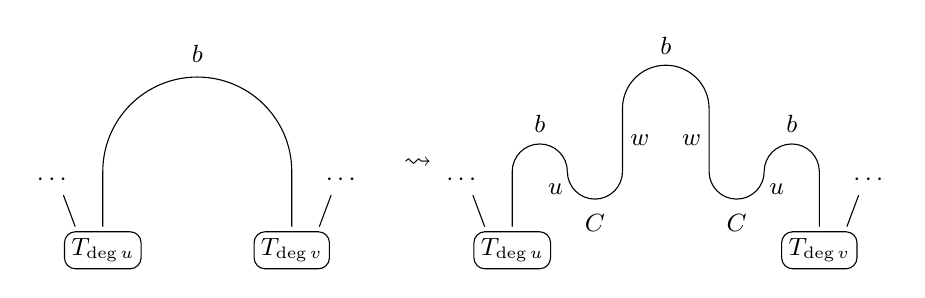
\begin{tikzpicture}[scale=1.0,
  box/.style={draw,rounded corners,inner sep=2.5pt,font=\small},
  lbl/.style={font=\small}]
  % ---------- before ----------
  \node[box] (TA) at (0,0) {$T_{\deg u}$};
  \node[box] (TB) at (2.4,0) {$T_{\deg v}$};
  \draw (0,0.3) -- (0,1.0) arc(180:0:1.2) -- (2.4,0.3);
  \node[lbl] at (1.2,2.5) {$b$};
  \draw (-0.35,0.3) -- (-0.5,0.7);
  \draw (2.75,0.3) -- (2.9,0.7);
  \node[lbl] at (-0.62,0.9) {$\cdots$};
  \node[lbl] at (3.05,0.9) {$\cdots$};
  % ---------- arrow ----------
  \node at (4.0,1.1) {$\leadsto$};
  % ---------- after ----------
  \begin{scope}[xshift=5.2cm]
    \node[box] (TC) at (0,0) {$T_{\deg u}$};
    \node[box] (TD) at (3.9,0) {$T_{\deg v}$};
    % left star wire + inserted cap + cup C
    \draw (0,0.3) -- (0,1.0) arc(180:0:0.35);         % inserted b
    \node[lbl] at (0.35,1.6) {$b$};
    \draw (0.7,1.0) arc(180:360:0.35);                 % cup C
    \node[lbl] at (1.05,0.35) {$\copair$};
    \node[lbl] at (0.55,0.78) {$u$};
    \node[lbl] at (1.62,1.4) {$w$};
    % left edge leg to central cap
    \draw (1.4,1.0) -- (1.4,1.8) arc(180:0:0.55) -- (2.5,1.0);
    \node[lbl] at (1.95,2.6) {$b$};
    % right cup C + inserted cap + star wire
    \draw (2.5,1.0) arc(360:180:0.0);                  % (join point)
    \draw (3.2,1.0) arc(360:180:0.35);                 % cup C
    \node[lbl] at (2.85,0.35) {$\copair$};
    \node[lbl] at (2.28,1.4) {$w$};
    \node[lbl] at (3.36,0.78) {$u$};
    \draw (3.9,0.3) -- (3.9,1.0) arc(0:180:0.35);      % inserted b
    \node[lbl] at (3.55,1.6) {$b$};
    % spare legs
    \draw (-0.35,0.3) -- (-0.5,0.7);
    \draw (4.25,0.3) -- (4.4,0.7);
    \node[lbl] at (-0.62,0.9) {$\cdots$};
    \node[lbl] at (4.55,0.9) {$\cdots$};
  \end{scope}
\end{tikzpicture}

\caption{The snake insertion on one edge. The inserted
evaluations pair each star leg with the mate leg $u$ of a
copairing, assembling the mates $\mate{T}$; the edge legs $w$ meet
the original evaluation and fuse to a single copairing by
Lemma~\ref{lemm:fusion}.}
\label{fig:snake}
\end{figure}

\subsection{Parity transfer}\label{subsec:paritytransfer}

The functional $h^{\mathrm{cat}}$ and the copairing $\copair$ do
not yet match the Regts--Sevenster normalisation, which uses the
twisted element. The discrepancy is a sign for each edge of the
odd sector, and it cancels against a compensating sign at the
vertices, as follows. First,
$h^{\mathrm{cat}}_{d}$ vanishes on
$\SymV^{a}V_{0}\otimes\Lambda^{j}V_{1}$ for $j$ odd, since
$T_{d}$ is even and $\beta_{d}$ is an even pairing. Define the
involution $\parinv$ on $\SymV V_{0}\otimes\Lambda V_{1}$ by
$\parinv\coloneqq(-1)^{j(j-1)/2}\cdot\mathrm{id}$ on the summand
of exterior degree $j$ --- for $j=2m$ this is $(-1)^{m}$, and the
odd-$j$ values are immaterial by the vanishing just noted --- and
set
\[
h^{\mathrm{RS}}\coloneqq h^{\mathrm{cat}}\circ\parinv .
\]

\begin{lemm}[Parity transfer]\label{lemm:paritytransfer}
For every closed graph $G$ without free circles,
\[
\mathrm{TN}_{h^{\mathrm{cat}},\copair}(G)
=\mathrm{TN}_{h^{\mathrm{RS}},\twistedC}(G).
\]
\end{lemm}

\begin{proof}
Expand both networks over the set $F$ of edges carrying the odd
part of the element ($\copair_{1}$ on the left, $\twistedC_{1}$
on the right); the even sectors agree term by term. Fix a
surviving term, and let $j_{v}\coloneqq\deg_{F}(v)$ be the number
of odd half-edges at $v$; terms with some $j_{v}$ odd vanish on
both sides by the odd-degree vanishing above, so every $j_{v}$ is
even. Replacing $h^{\mathrm{cat}}$ by $h^{\mathrm{RS}}$
multiplies the term by
$\prod_{v}(-1)^{j_{v}/2}=(-1)^{\frac12\sum_{v}j_{v}}
=(-1)^{|F|}$, by the handshake identity
$\sum_{v}\deg_{F}(v)=2|F|$, which is valid for loops precisely
because a loop contributes two half-edges. Replacing
$\copair_{1}$ by $\twistedC_{1}=-\copair_{1}$ multiplies the term
by $(-1)^{|F|}$ as well. The two factors cancel.
\end{proof}

A warning about presentations. The involution $\parinv$ is
calibrated against the $\kappa$-paired form of the vertex
argument fixed in Section~\ref{subsec:mpf}. A presentation that
instead lists the odd factors in some canonical colour order
generates Koszul reordering signs of its own, and the twist must
then be recomputed against that presentation rather than carried
over unchanged: mixing the two conventions changes every Eulerian
summand by exactly $(-1)^{|F|}$ --- the sign at stake in
Lemma~\ref{lemm:paritytransfer}. The loop example of
Section~\ref{subsec:mpf} serves as the convention check: such a
mixture flips its odd sector from $-2$ to $+2$.

%%%%%%%%%%%%%%%%%%%%%%%%%%%%%%%%%%%%%%%%%%%%%%%%%%%%%%%%%%%%%%%%%%%%%%
\section{The circuit expansion and the Regts--Sevenster
formula}\label{sec:circuit}
%%%%%%%%%%%%%%%%%%%%%%%%%%%%%%%%%%%%%%%%%%%%%%%%%%%%%%%%%%%%%%%%%%%%%%

Two tasks remain: to prove that the twisted tensor network of
Section~\ref{sec:extraction} is \emph{exactly} the Regts--Sevenster
sum of Definition~5, circuit signs included; and to assemble the
proof of the Main Theorem. The first
part is a statement about super linear algebra alone --- no
connection category enters --- and we state it as a theorem in its
own right, since it is the step that turns an abstract fibre
functor into the concrete model of \cite{RS21}.

\begin{theo}[Reconstruction]\label{theo:reconstruction}
Let $V=V_{0}\oplus V_{1}$ be a finite-dimensional super vector
space with a nondegenerate supersymmetric even bilinear form $b$,
coordinatised as in Section~\ref{subsec:formcoords}, let
$\twistedC$ be the twisted element, and let $h=(h_{d})$ be
functionals on the super symmetric powers of $V$ vanishing in odd
exterior degree. Then for every graph $G$ without free circles,
\[
\mathrm{TN}_{h,\twistedC}(G)=p_{h}(G),
\]
the right-hand side being the sum of Definition~5 in
Section~\ref{subsec:mpf}.
\end{theo}

The proof occupies
Sections~\ref{subsec:reduction}--\ref{subsec:circuitproof}. The
strategy is to expand the twisted element into its even and odd
parts, observe that the even part is diagonal and reproduces the
colouring sum over $\psi$, and reduce the odd part to a sign
computation along each circuit; the computation is carried out for
a single circuit and shown to be insensitive to everything else.

\subsection{The reduction}\label{subsec:reduction}

In the edge order fixed for the network, expand each factor as
$\twistedC=\twistedC_{0}+\twistedC_{1}$ and distribute:
\[
\bigotimes_{e\in E}\twistedC
=\sum_{F\subseteq E}\;
\bigotimes_{e\in E}\twistedC_{\mathbf{1}_{F}(e)},
\]
where $\mathbf{1}_{F}$ is the characteristic function of $F$, so
the $F$-summand carries $\twistedC_{1}$ on the edges of $F$ and
$\twistedC_{0}$ elsewhere; both parts being even tensors, the
regroupings below introduce no sign on this account.
The even part $\twistedC_{0}=\copair_{0}=\sum_{i}e_{i}\otimes
e_{i}$ is diagonal, and its legs contribute, at each vertex, the
word of $e_{\psi(a)}$ over the half-edges
$a\in\halfedges{E\setminus F}{v}$, summed over colourings $\psi$
of the edges of $E\setminus F$; this is precisely the
$\psi$-sum of Definition~5. Since each $h_{d}$ vanishes in odd
exterior degree, a term survives only if every vertex receives an
even number of odd half-edges, i.e.\ only if $F$ is Eulerian.
For Eulerian $F$, choose an Eulerian orientation and a compatible
local pairing $\kappa$, as in
Section~\ref{subsec:mpf}; by \cite[Proposition~3]{RS21} the
right-hand side of the Reconstruction Theorem does not depend on
these choices. (The dependence is in any case illusory here: the
argument below applies to an arbitrary choice, and its conclusion
--- equality with the manifestly choice-free left-hand side ---
re-derives this independence for the graphs at hand.) By Lemma~\ref{lemm:TNinv} we may also choose the
half-edge order at each vertex so that the even legs occur first
and the odd legs occur in $\kappa$-paired order; the even and odd
legs then combine through the quotient map without interaction:
for even vectors $e_{i_{1}},\dotsc,e_{i_{a}}$ and odd vectors
$x_{1},y_{1},\dotsc,x_{m},y_{m}$,
\begin{equation}\label{eq:mixedquotient}
\symq{d}\bigl(e_{i_{1}}\otimes\dotsb\otimes e_{i_{a}}
\otimes x_{1}\otimes y_{1}\otimes\dotsb\otimes x_{m}\otimes
y_{m}\bigr)
=(e_{i_{1}}\odot\dotsb\odot e_{i_{a}})\otimes
(x_{1}\wedge y_{1})\wedge\dotsb\wedge(x_{m}\wedge y_{m})
\end{equation}
under the isomorphism
$\SymV_{s}V\cong\SymV V_{0}\otimes\Lambda V_{1}$: moving even legs
past odd legs costs no sign, no factorial normalisation appears,
and the right-hand side is exactly the vertex argument of
Definition~5. Write $\mathrm{Regroup}_{F,\kappa}$ for the
restriction of $\mathrm{Regroup}_{G}$ to the odd legs, targeting
the $\kappa$-paired vertex--half-edge order. The theorem then
reduces to the following identity, applied circuit by circuit.

\subsection{The twisted element as maps}\label{subsec:twistedmaps}

\begin{lemm}\label{lemm:twistedmaps}
In the coordinates of Section~\ref{subsec:formcoords}:
\begin{enumerate}
\item[(i)] $\twistedC_{1}
  =-\sum_{i}\xi_{i}\otimes\eta_{i}
  =\sum_{i}\eta_{i}\otimes\xi_{i}$;
\item[(ii)] $b(\eta_{i},\xi_{j})=\delta_{ij}$ for all $i,j$, and
  consequently $L_{\copair}=\mathrm{id}_{V}$ and
  $L_{\twistedC}=\parityop$.
\end{enumerate}
\end{lemm}

\begin{proof}
(i) The first equality is the definition of
$\twistedC=(\parityop\otimes\mathrm{id})\copair$. For the second,
each $\eta_{i}$ is a signed $\xi$, and unwinding the definition
gives
$\sum_{i}\eta_{i}\otimes\xi_{i}
=\sum_{m\le\ell}\bigl(-\xi_{m+\ell}\otimes\xi_{m}
+\xi_{m}\otimes\xi_{m+\ell}\bigr)
=-\sum_{i}\xi_{i}\otimes\eta_{i}$.
(ii) For $i\le\ell$:
$b(\eta_{i},\xi_{j})=-b(\xi_{i+\ell},\xi_{j})
=-(-\delta_{ij})=\delta_{ij}$; for $i>\ell$:
$b(\eta_{i},\xi_{j})=b(\xi_{i-\ell},\xi_{j})=\delta_{ij}$, using
$b(\xi_{m},\xi_{m+\ell})=1$. Hence
$L_{\copair_{1}}(\xi_{j})=\sum_{i}\xi_{i}\,b(\eta_{i},\xi_{j})
=\xi_{j}$, while
$L_{\copair_{0}}(e_{j})=e_{j}$ directly, and the cross-parity
terms vanish because $b$ is even; so
$L_{\copair}=\mathrm{id}_{V}$, and
$\twistedC_{1}=-\copair_{1}$ gives $L_{\twistedC}=\parityop$.
\end{proof}

\subsection{The circuit sign}\label{subsec:circuitproof}

Consider a single $\kappa$-circuit of length $n$: edges
$a_{1},\dotsc,a_{n}$ traversed in order through
vertices $v_{1},\dotsc,v_{n}$, the head half-edge $x_{j}$ of
$a_{j}$ landing in the in-slot of $v_{j}$ and the tail half-edge
$y_{j}$ in the out-slot of $v_{j-1}$ (indices modulo $n$).

\begin{lemm}\label{lemm:cyclicparity}
The permutation from the edge-wise word
$(x_{1},y_{1},x_{2},y_{2},\dotsc,x_{n},y_{n})$ to the vertex-wise
word $(x_{1},y_{2}\,|\,x_{2},y_{3}\,|\,\dotsc\,|\,x_{n},y_{1})$
fixes the positions $1,3,\dotsc,2n-1$ and acts on the positions
$2,4,\dotsc,2n$ as a
single $n$-cycle. All $2n$ legs being odd, its Koszul sign is
$(-1)^{n-1}$.
\end{lemm}

\begin{proof}
The $x_{j}$ occupy the positions $1,3,\dotsc,2n-1$ in both
words, in the same
order; the $y$'s move by one step of a cyclic rotation, which is
an $n$-cycle on the remaining positions, of sign $(-1)^{n-1}$; by
Lemma~\ref{lemm:koszul} the Koszul sign of a rearrangement of an
all-odd word is the sign of the permutation. We illustrate the
two words in Figure~\ref{fig:circuit}.
\end{proof}

\begin{figure}
\centering
% fig_circuit.tex -- edge-wise vs vertex-wise words on a length-3
% circuit; the y's rotate by one step (a 3-cycle on even positions).
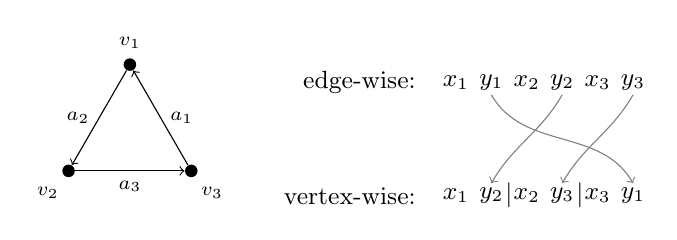
\begin{tikzpicture}[scale=0.9,
  vert/.style={circle,fill,inner sep=1.6pt},
  l/.style={inner sep=1.5pt,font=\small}]
  % the oriented triangle
  \node[vert] (v1) at (90:1) {};
  \node[vert] (v2) at (210:1) {};
  \node[vert] (v3) at (330:1) {};
  \draw[->] (v1) -- node[left,font=\scriptsize] {$a_{2}$} (v2);
  \draw[->] (v2) -- node[below,font=\scriptsize] {$a_{3}$} (v3);
  \draw[->] (v3) -- node[right,font=\scriptsize] {$a_{1}$} (v1);
  \node[font=\scriptsize,above] at (v1.north) {$v_{1}$};
  \node[font=\scriptsize,below left] at (v2.south) {$v_{2}$};
  \node[font=\scriptsize,below right] at (v3.south) {$v_{3}$};
  % the two words, one node per letter
  \begin{scope}[xshift=3.1cm,yshift=0.75cm]
    \node[l,anchor=east] at (1.0,0) {edge-wise:};
    \node[l] (ty1) at (2.0,0) {$y_{1}$};
    \node[l] (tx1) at (1.5,0) {$x_{1}$};
    \node[l] (tx2) at (2.5,0) {$x_{2}$};
    \node[l] (ty2) at (3.0,0) {$y_{2}$};
    \node[l] (tx3) at (3.5,0) {$x_{3}$};
    \node[l] (ty3) at (4.0,0) {$y_{3}$};
    \node[l,anchor=east] at (1.0,-1.6) {vertex-wise:};
    \node[l] (bx1) at (1.5,-1.6) {$x_{1}$};
    \node[l] (by2) at (2.0,-1.6) {$y_{2}$};
    \node[l] at (2.25,-1.6) {$|$};
    \node[l] (bx2) at (2.5,-1.6) {$x_{2}$};
    \node[l] (by3) at (3.0,-1.6) {$y_{3}$};
    \node[l] at (3.25,-1.6) {$|$};
    \node[l] (bx3) at (3.5,-1.6) {$x_{3}$};
    \node[l] (by1) at (4.0,-1.6) {$y_{1}$};
    \draw[->,gray] (ty1.south) to[out=-60,in=120] (by1.north);
    \draw[->,gray] (ty2.south) to[out=-120,in=60] (by2.north);
    \draw[->,gray] (ty3.south) to[out=-120,in=60] (by3.north);
  \end{scope}
\end{tikzpicture}

\caption{Edge-wise and vertex-wise words on a circuit of length
three.}
\label{fig:circuit}
\end{figure}
\FloatBarrier

Three small auxiliaries dispose of the interactions between
circuits. First, the quotient map sends an interleaved product of
odd pairs to the wedge --- the all-odd case of
\eqref{eq:mixedquotient}. Second, each pair
$x\wedge y$ of odd vectors is an even block, so reordering local
pairs at a vertex, and moving complete circuit blocks past one
another --- including circuits sharing a vertex --- introduces no
sign. Third, each factor $\twistedC_{1}$ is a sum of terms with
two odd legs, hence an even block, so reordering the factors of
$\twistedC_{1}^{\otimes|F|}$ into circuit-consecutive order costs
no sign; the edge order in Lemma~\ref{lemm:cyclicparity} may
therefore be assumed circuit-consecutive.\footnote{This
normalisation is the only point at which the circuit
decomposition enters the proof, and it can be avoided: writing
$W$ for the walk permutation of the half-edges of $F$ determined
by $\kappa$ and the orientation, the orbits of
$W|_{\mathrm{out}}$, its restriction to outgoing half-edges, are
the circuits, so
$\operatorname{sgn}(W|_{\mathrm{out}})=(-1)^{|F|-c(\kappa)}$,
i.e.\ $(-1)^{c(\kappa)}=(-1)^{|F|}
\operatorname{sgn}(W|_{\mathrm{out}})$; the total regrouping
parity is the same permutation sign, and the two combine as in
Lemma~\ref{lemm:circuitsign} with no decomposition into circuits.
We keep the circuitwise proof for its transparency.}

\begin{lemm}\label{lemm:circuitsign}
With notation as above,
\[
\Bigl(\bigotimes_{v}\symq{\deg_{F}v}\Bigr)\circ
\mathrm{Regroup}_{F,\kappa}
\bigl(\twistedC_{1}^{\otimes|F|}\bigr)
=(-1)^{c(\kappa)}
\sum_{\varphi\colon F\to[2\ell]}\;
\bigotimes_{v}\bigwedge_{(a_{1},a_{2})\in\kappa_{v}}
\xi_{\varphi(a_{1})}\wedge\eta_{\varphi(a_{2})} .
\]
\end{lemm}

\begin{proof}
By the third auxiliary the edge factors are in
circuit-consecutive order, and by the second the identity
factors over the circuits of $\kappa$; fix one circuit, of length
$n$. Writing each of its edge factors as
$\twistedC_{1}=-\sum_{i}\xi_{i}\otimes\eta_{i}$
(Lemma~\ref{lemm:twistedmaps}(i)), with the head leg carrying
$\xi$ and the tail leg carrying $\eta$ --- an assignment licensed
by the supersymmetry of $\twistedC$
(Section~\ref{subsec:copairing}) --- the $n$ edge factors
contribute the sign $(-1)^{n}$ in total. The regrouping to the
vertex-wise word contributes $(-1)^{n-1}$
(Lemma~\ref{lemm:cyclicparity}). The resulting vertex-wise word
is $\bigotimes_{j}\xi_{\varphi(a_{j})}\otimes
\eta_{\varphi(a_{j+1})}$, constant colourings and mixed
colourings alike being carried along; the quotient maps convert
it to the displayed wedges by the first auxiliary, with no
further sign. The total sign per circuit is
$(-1)^{n}(-1)^{n-1}=-1$, independent of $n$, giving
$(-1)^{c(\kappa)}$ overall. Loops are the case $n=1$ and pairs of
parallel edges the case $n=2$; the half-edge conventions of
Section~\ref{subsec:graphs} make both cases instances of the
general computation, with nothing further to check.
\end{proof}

\begin{proof}[Proof of the Reconstruction Theorem]
Combine Lemma~\ref{lemm:circuitsign} with the reduction of
Section~\ref{subsec:reduction}: for each Eulerian $F$, the odd
sector produces the sign $(-1)^{c(\kappa)}$ together with the
$\varphi$-sum of wedges, the even sector produces the
$\psi$-sum, and applying the functionals $h_{\deg v}$ at the
vertices yields exactly the summand of Definition~5 for $F$.
\end{proof}

The loop example of Section~\ref{subsec:mpf} keeps its promise
here. For the loop graph $L$, the odd sector of
$\mathrm{TN}_{h,\twistedC}(L)$ is the case $n=1$ of
Lemma~\ref{lemm:circuitsign}: the single edge factor
$\twistedC_{1}$ contributes $(-1)^{1}$, the cyclic regrouping is
the identity permutation, of sign $(-1)^{0}$, and the product is
the per-circuit $-1$; the $\varphi$-sum then passes through the
common wedge $\xi_{\varphi}\wedge\eta_{\varphi}$ for both odd
colours, while the even sector contributes
$h(e_{\psi}\odot e_{\psi})$. The network thus reproduces, term by
term, the hand computation of Section~\ref{subsec:mpf}.

\subsection{Multiplicativity, circles, and the proof of the Main
Theorem}\label{subsec:assembly}

Definition~5 is multiplicative over disjoint union: the Eulerian
subset, both colourings, and the local circuit data of a disjoint
union all split componentwise, and $c(\kappa)$ is additive; the
circle convention extends this to graphs with free circles.

\begin{proof}[Proof of the Main Theorem]
The implication from mixed partition functions to exponentially
bounded rank is \cite[Theorem~6]{RS21}. For the converse, let $f$
satisfy (H1) and (H2). Write an arbitrary graph
as $G=G^{\circ}\sqcup\freecircle^{\,r}$ with $G^{\circ}$ free of
circles. Then
\begin{align*}
f(G)&=f(G^{\circ})\,f(\freecircle)^{r}
&&\text{(Lemma~\ref{lemm:mult})}\\
&=(k-2\ell)^{r}\,
\mathrm{TN}_{h^{\mathrm{cat}},\copair}(G^{\circ})
&&\text{(Section~\ref{subsec:copairing},
Lemma~\ref{lemm:indexraising})}\\
&=(k-2\ell)^{r}\,
\mathrm{TN}_{h^{\mathrm{RS}},\twistedC}(G^{\circ})
&&\text{(Lemma~\ref{lemm:paritytransfer})}\\
&=(k-2\ell)^{r}\,p_{h^{\mathrm{RS}}}(G^{\circ})
&&\text{(the Reconstruction Theorem)}\\
&=p_{h^{\mathrm{RS}}}(G)
&&\text{(circle convention),}
\end{align*}
so $f=p_{h^{\mathrm{RS}}}$ is a mixed partition function on
$\mathbb{C}^{k|2\ell}$, and $k,2\ell\le\lfloor 2eR\rfloor$ by
Corollary~\ref{coro:dimbound}.
\end{proof}

%%%%%%%%%%%%%%%%%%%%%%%%%%%%%%%%%%%%%%%%%%%%%%%%%%%%%%%%%%%%%%%%%%%%%%
\section{Consequences and final remarks}\label{sec:consequences}
%%%%%%%%%%%%%%%%%%%%%%%%%%%%%%%%%%%%%%%%%%%%%%%%%%%%%%%%%%%%%%%%%%%%%%

We close with an observation, a remark, and a taking of stock.

\begin{obse}[The ordinary case]\label{obse:ordinary}
If some super exterior power of $\genX$ vanishes in $\cauchy$ ---
that is, $\Phi_{n}(e_{(1^{n})})=0$ for some $n\ge1$ --- then
$V_{1}=0$, and $f$ is an ordinary edge-colouring model.
\end{obse}

\begin{proof}
Applying $\fib$ as in the proof of
Corollary~\ref{coro:dimbound} gives $\Lambda_{s}^{n}V=0$, where
$\Lambda_{s}$ denotes the super exterior power. But
$\Lambda_{s}^{n}V\cong\bigoplus_{i+j=n}\Lambda^{i}V_{0}\otimes
\SymV^{j}V_{1}$, and if $V_{1}\ne0$ the summand $i=0$, $j=n$ is
nonzero for every $n$. Hence $V_{1}=0$, the model has no odd
colours, every subset $F\ne\emptyset$ contributes nothing, and
$p_{h}$ reduces to an ordinary edge-colouring partition
function.
\end{proof}

In this way the characterisation theorem of \cite{Sch15} for
ordinary edge-colouring models sits inside
the Main Theorem as the sector in which an exterior power
dies; we have not attempted a precise translation between this
condition and the real-valuedness hypotheses of \cite{Sch15},
which would take us too far afield.

Finally, we take stock. Before the Main Theorem, exponentially
bounded edge-connection rank was a necessary condition for being
a mixed partition function; it is now the defining one, and the
ordinary/skew/mixed family of edge-colouring models closes at the
boundary that rank condition draws. The proof has two working parts, and neither is
specific to this conjecture: the connection category turns rank
conditions on graph parameters into growth conditions on a tensor
category, where structural results such as \cite{EP26} apply; and
the reconstruction theorem turns the abstract output of Deligne's
theorem back into the concrete normalisations of a combinatorial
model. It is the author's hope that both will find further use
beyond the theorem proved here.

%%%%%%%%%%%%%%%%%%%%%%%%%%%%%%%%%%%%%%%%%%%%%%%%%%%%%%%%%%%%%%%%%%%%%%
\appendix
\section[Rational trace zeta functions from exponential
endomorphism growth]{Rational trace zeta functions\texorpdfstring{\\}{ }from
exponential endomorphism growth}\label{app:zeta}
%%%%%%%%%%%%%%%%%%%%%%%%%%%%%%%%%%%%%%%%%%%%%%%%%%%%%%%%%%%%%%%%%%%%%%

This appendix has two aims: to prove, by a direct
symmetric-function argument, that
exponential endomorphism growth makes the trace zeta function of
every endomorphism rational, with explicit degree bounds; and
thereby to give a proof of the nilpotent-trace step of
Section~\ref{sec:semisimple} that is independent of
\cite{EP26}. Nothing in this appendix depends on
Sections~\ref{sec:semisimple}--\ref{sec:circuit} or on the
citations made there; the only inputs are the classical
representation theory of symmetric groups and some symmetric
function theory, for which we cite
\cite{Sag01,Mac95,FH91}, and the standard trace calculus of rigid
symmetric categories (cyclicity, multiplicativity over $\otimes$,
and $\tr(c\circ(u\otimes v))=\tr(uv)$; see
e.g.\ \cite[\S4.7]{EGNO15}), which for the connection category
was proved combinatorially in Lemma~\ref{lemm:tracecalc}.

\subsection{Statement}\label{subsec:appstatement}

Throughout the appendix, $\mathcal{C}$ is a rigid symmetric
$\mathbb{C}$-linear monoidal category with
$\End(\unitobj)=\mathbb{C}$, and $Z$ is an object of $\mathcal{C}$
satisfying
\begin{equation}\label{eq:growth}
\dim\End(Z^{\otimes n})\le A^{n}\qquad(n\ge 0)
\end{equation}
for a real constant $A\ge 1$. For $g\in\End(Z)$ we write
$\tau_{m}\coloneqq\tr(g^{m})$ and define the \emph{trace zeta
function}
\[
\tzeta{g}(z)\coloneqq
\exp\Bigl(\sum_{m\ge1}\frac{\tau_{m}}{m}\,z^{m}\Bigr)
\in\mathbb{C}[[z]].
\]

\begin{theo}\label{theo:zeta}
Let $s$ be any integer with $s>2e\sqrt{A}$. Then for every
$g\in\End(Z)$ the trace zeta function is rational,
\[
\tzeta{g}(z)=\frac{P_{g}(z)}{Q_{g}(z)}
\qquad\text{with}\qquad
\deg P_{g}\le s-1,\quad \deg Q_{g}\le s-1,
\]
where $P_{g}$ and $Q_{g}$ are coprime polynomials with constant
term~$1$. Equivalently, there are disjoint multisets of nonzero
complex numbers $\{\alpha_{1},\dotsc,\alpha_{a'}\}$ and
$\{\beta_{1},\dotsc,\beta_{b'}\}$ with $a',b'\le s-1$ and
\[
\tau_{m}=\sum_{i=1}^{a'}\alpha_{i}^{m}
-\sum_{j=1}^{b'}\beta_{j}^{m}
\qquad(m\ge1).
\]
\end{theo}

We call the pair of multisets the \emph{super-spectrum} of $g$: it
is defined as the root data of $P_{g}$ and $Q_{g}$, and we do not
claim that its members are eigenvalues of $g$ in any further sense.

\begin{coro}\label{coro:nilpotent}
Every nilpotent $g\in\End(Z)$ has $\tr(g)=0$; indeed
$\tau_{m}=0$ for all $m\ge1$.
\end{coro}

Etingof and Penneys \cite{EP26}, whose theorem
Section~\ref{sec:semisimple} uses, work in the broader braided
setting and prove a structural theorem: non-negligible objects of
moderate growth are rigid, nilpotent quantum traces vanish, and a
semisimplification exists. The present result is symmetric and
objectwise --- it concerns one dualizable object at a time, with
no Cauchy completeness, no trace nondegeneracy and no fibre
functor entering --- and by a direct symmetric-function argument
it proves more in that setting: the full super-spectrum of every
endomorphism, with degree bounds explicit in the growth constant,
and an elementary explanation of \emph{why} nilpotent traces
vanish. We have not
found the quantitative objectwise formulation of
Theorem~\ref{theo:zeta} in the literature; the closely related
prior work is discussed in
Section~\ref{subsec:appliterature}.

The question answered by Corollary~\ref{coro:nilpotent} has some
history. Andr\'e and Kahn write, at the opening of
\cite[\S7.3]{AK02}: ``\emph{Nous ignorons si un endomorphisme
nilpotent est toujours de trace nilpotente, sans hypoth\`ese
suppl\'ementaire}.'' Affirmative answers were previously available
under Kimura-finiteness \cite[Thm~9.2.2, Prop~7.3.3]{AK02}, in the
presence of a fibre functor to an abelian rigid target
\cite[Prop~7.3.3]{AK02}, and now in braided categories of moderate
growth \cite{EP26}. Corollary~\ref{coro:nilpotent} gives an
independent quantitative proof in the objectwise
exponential-growth setting, without invoking a fibre functor, a
Kimura decomposition, or the semisimplification machinery.

\subsection{Fat-hook confinement}\label{subsec:fathook}

We use the standard representation theory of the symmetric group
$S_{n}$ over $\mathbb{C}$ \cite{Sag01,FH91}: the group algebra
decomposes into simple blocks
$\mathbb{C}[S_{n}]=\bigoplus_{\lambda\vdash n}B_{\lambda}$ with
$B_{\lambda}\cong\mathrm{Mat}_{d_{\lambda}}(\mathbb{C})$, indexed
by partitions $\lambda$ of $n$ with irreducible dimensions
$d_{\lambda}$; the central primitive idempotent of $B_{\lambda}$ is
\[
e_{\lambda}
=\frac{d_{\lambda}}{n!}\sum_{\pi\in S_{n}}\chi_{\lambda}(\pi)\,\pi .
\]
The symmetric braiding makes $S_{n}$ act on $Z^{\otimes n}$, giving
an algebra homomorphism $\Phi_{n}$ from $\mathbb{C}[S_{n}]$ to
$\End(Z^{\otimes n})$. We say the
partition $\lambda$ \emph{survives} if
$\Phi_{n}(e_{\lambda})\ne 0$, and \emph{dies} otherwise. Since
$\ker\Phi_{n}$ is a two-sided ideal, hence a sum of blocks, the
whole block $B_{\lambda}$ of a surviving $\lambda$ embeds into
$\End(Z^{\otimes n})$; this is the entire mechanism by which
\eqref{eq:growth} acts.

\begin{lemm}\label{lemm:blockdeath}
If $\lambda\vdash n$ survives, then $d_{\lambda}^{2}\le A^{n}$.
\end{lemm}

\begin{proof}
The block $B_{\lambda}\cong\mathrm{Mat}_{d_{\lambda}}(\mathbb{C})$
embeds into $\End(Z^{\otimes n})$, whose dimension is at most
$A^{n}$ by \eqref{eq:growth}.
\end{proof}

\begin{lemm}\label{lemm:upward}
Death is upward closed: if $\lambda\vdash n$ dies and
$\lambda\subseteq\mu\vdash n+m$, then $\mu$ dies.
\end{lemm}

\begin{proof}
We first record the branching containment: if
$\lambda\subseteq\mu$ then the irreducible $V_{\lambda}$ appears in
the restriction of $V_{\mu}$ to $S_{n}$. Indeed, nested Young
diagrams are joined by a chain
$\lambda=\nu_{0}\subset\nu_{1}\subset\dotsb\subset\nu_{m}=\mu$
adding one box at a time; the branching rule
\cite[Thm~2.8.3]{Sag01} gives that $V_{\nu_{i}}$ appears in the
restriction of $V_{\nu_{i+1}}$ to the next symmetric group down,
and ``appears in the restriction'' is transitive by
semisimplicity.

Consequently the element
$e_{\mu}(e_{\lambda}\otimes 1_{m})e_{\mu}$ of the simple block
$B_{\mu}\subseteq\mathbb{C}[S_{n+m}]$ is nonzero: it is the
compression to $V_{\mu}$ of the projection onto the
$\lambda$-isotypic part of the restriction, which is a nonzero
operator by the previous paragraph. If $\mu$ survived, then
$\Phi_{n+m}$ would be injective on $B_{\mu}$, so
$\Phi_{n+m}\bigl(e_{\mu}(e_{\lambda}\otimes1)e_{\mu}\bigr)\ne0$;
but
$\Phi_{n+m}(e_{\lambda}\otimes1)
=\Phi_{n}(e_{\lambda})\otimes\mathrm{id}=0$
since $\lambda$ dies. This contradiction proves the lemma.
\end{proof}

\begin{lemm}\label{lemm:squaredeath}
Let $s$ be an integer with $s>2e\sqrt{A}$. Then the square
partition $(s^{s})$ dies.
\end{lemm}

\begin{proof}
Every hook length of the square $(s^{s})$ is less than $2s$, so
the hook length formula and $n!\ge(n/e)^{n}$ --- one term of the
series $e^{n}=\sum_{k}n^{k}/k!$ --- give, with $n=s^{2}$,
\[
\log d_{(s^{s})}
\ge \log\frac{(s^{2})!}{(2s)^{s^{2}}}
\ge s^{2}\bigl(\log s-1-\log 2\bigr).
\]
The hypothesis $s>2e\sqrt{A}$ says precisely that
$\log s-1-\log2>\tfrac12\log A$, whence
$d_{(s^{s})}^{2}>A^{s^{2}}$, and Lemma~\ref{lemm:blockdeath} kills
$(s^{s})$. We have made no attempt to optimise the constant.
\end{proof}

For integers $a,b\ge0$ let
$\hook{a}{b}\coloneqq\{\lambda:\lambda_{a+1}\le b\}$ denote the
\emph{fat hook}: the set of partitions whose Young diagram fits in
the union of $a$ rows and $b$ columns
(Figure~\ref{fig:fathook}). A partition lies outside
$\hook{a}{b}$ if and only if it contains the rectangle
$\bigl((b+1)^{a+1}\bigr)$.

\begin{figure}
\centering
% fig_fathook.tex -- the fat hook H(a,b) and a dead square (s^s).
% Drawn with a = 2, b = 3, s = 5: the top band is the a unbounded
% rows, the left band the b unbounded columns; the square pokes out
% of both arms.
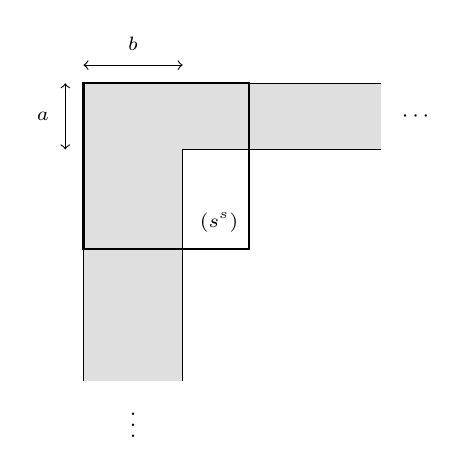
\begin{tikzpicture}[scale=0.42]
  % shaded arms
  \fill[gray!25] (0,0) rectangle (9,-2);
  \fill[gray!25] (0,0) rectangle (3,-9);
  % hook boundary (outer edges and inner staircase)
  \draw (9,0) -- (0,0) -- (0,-9);
  \draw (9,-2) -- (3,-2) -- (3,-9);
  % unboundedness marks
  \node[font=\footnotesize] at (10.1,-1) {$\cdots$};
  \node[font=\footnotesize] at (1.5,-10.1) {$\vdots$};
  % extent markers for a (rows) and b (columns)
  \draw[<->] (-0.55,0) -- (-0.55,-2);
  \node[font=\scriptsize,left] at (-0.75,-1) {$a$};
  \draw[<->] (0,0.55) -- (3,0.55);
  \node[font=\scriptsize,above] at (1.5,0.7) {$b$};
  % the dead square
  \draw[thick] (0,0) rectangle (5,-5);
  \node[font=\scriptsize] at (4.1,-4.2) {$(s^{s})$};
\end{tikzpicture}

\caption{The fat hook $\hook{a}{b}$ and a dead square.}
\label{fig:fathook}
\end{figure}
\FloatBarrier

\begin{coro}\label{coro:hookconfine}
With $s$ as in Lemma~\ref{lemm:squaredeath}, every surviving
partition lies in the fat hook $\hook{s-1}{s-1}$.
\end{coro}

\begin{proof}
A partition outside $\hook{s-1}{s-1}$ contains the square
$(s^{s})$, which dies; apply Lemma~\ref{lemm:upward}.
\end{proof}

We now convert confinement into a statement about traces. For a
permutation $\pi$ with cycle lengths $c_{1},\dotsc,c_{r}$, the
standard trace calculus recalled at the head of this appendix
gives, by induction on the cycles,
\begin{equation}\label{eq:cyclefact}
\tr\bigl(\Phi_{n}(\pi)\circ g^{\otimes n}\bigr)
=\prod_{i=1}^{r}\tau_{c_{i}} .
\end{equation}
Indeed, each cycle of $\pi$ threads the corresponding tensor
factors of $g^{\otimes n}$ into a single power of $g$, closed
into a trace.
For a partition $\lambda\vdash n$, write $s_{\lambda}[\tau]$ for
the Schur polynomial in the power sums evaluated at
$p_{m}\mapsto\tau_{m}$; concretely, define
$h_{0}\coloneqq1$, $h_{n}\coloneqq0$ for $n<0$, and
$nh_{n}\coloneqq\sum_{i=1}^{n}\tau_{i}h_{n-i}$ by Newton's
identities, and
$s_{\lambda}[\tau]\coloneqq
\det\bigl(h_{\lambda_{i}-i+j}\bigr)_{1\le i,j\le r}$, with $r$
the number of parts of $\lambda$, by Jacobi--Trudi
\cite[Chapter~I]{Mac95}.

\begin{lemm}[Frobenius formula]\label{lemm:frobenius}
For every $\lambda\vdash n$,
\[
\tr\bigl(\Phi_{n}(e_{\lambda})\circ g^{\otimes n}\bigr)
=d_{\lambda}\cdot s_{\lambda}[\tau].
\]
In particular, if $\lambda$ dies then $s_{\lambda}[\tau]=0$.
\end{lemm}

\begin{proof}
Expand $e_{\lambda}$ and apply \eqref{eq:cyclefact} to each term:
writing $z_{\mu}$ for the order of the centraliser of a
permutation of cycle type $\mu$, so that the number of such
permutations is $n!/z_{\mu}$,
\begin{align*}
\tr\bigl(\Phi_{n}(e_{\lambda})\circ g^{\otimes n}\bigr)
&=\frac{d_{\lambda}}{n!}\sum_{\pi}\chi_{\lambda}(\pi)
  \prod_{i}\tau_{c_{i}(\pi)}
 =d_{\lambda}\sum_{\mu\vdash n}z_{\mu}^{-1}\chi_{\lambda}(\mu)\,
  p_{\mu}[\tau]
 =d_{\lambda}\,s_{\lambda}[\tau],
\end{align*}
the last step by the Frobenius characteristic formula
$s_{\lambda}=\sum_{\mu}z_{\mu}^{-1}\chi_{\lambda}(\mu)p_{\mu}$
\cite[I.7]{Mac95}. If $\lambda$ dies, the left-hand side is the
trace of the zero morphism composed with $g^{\otimes n}$, and
$d_{\lambda}\ne0$.
\end{proof}

Combining Corollary~\ref{coro:hookconfine} with
Lemma~\ref{lemm:frobenius}: for every $g\in\End(Z)$,
\begin{equation}\label{eq:hookvanishing}
s_{\lambda}[\tau]=0
\qquad\text{for every }\lambda\notin \hook{s-1}{s-1}.
\end{equation}

\subsection{Rationality of hook-confined
sequences}\label{subsec:rationality}

The passage from \eqref{eq:hookvanishing} to
Theorem~\ref{theo:zeta} is a piece of classical symmetric function
theory. The rationality criterion involved goes back to Borel
\cite{Bor1894}; the formulation through
vanishing Hankel determinants is the determinantal rationality
of Larsen and Lunts \cite[\S2]{LL04}, and the assembly via
Jacobi--Trudi, in the equivalent language of $\lambda$-rings, is
due to Mazza and Weibel \cite[Prop.~4.14, Cor.~4.15]{MW13}. We
include a self-contained proof, partly to keep the appendix
elementary and partly because we want the sharp hook-shaped degree
bounds; the argument is a Jacobi--Trudi null-vector computation.

\begin{lemm}\label{lemm:sfrationality}
Let $(\tau_{m})_{m\ge1}$ be a complex sequence with
$s_{\lambda}[\tau]=0$ for every $\lambda\notin\hook{a}{b}$. Then
there are coprime polynomials $P$ and $Q$ with constant term $1$,
$\deg P\le b$ and $\deg Q\le a$, such that
$H(z)\coloneqq\sum_{n\ge0}h_{n}z^{n}=P(z)/Q(z)$; consequently,
factoring $Q(z)=\prod_{i}(1-\alpha_{i}z)$ and
$P(z)=\prod_{j}(1-\beta_{j}z)$, we have
$\tau_{m}=\sum_{i}\alpha_{i}^{m}-\sum_{j}\beta_{j}^{m}$, where
the $\alpha_{i}$ and the $\beta_{j}$ form disjoint multisets of
nonzero numbers of sizes at most $a$ and $b$ respectively.
\end{lemm}

\begin{proof}
For strictly decreasing integers
$\rho_{1}>\dotsb>\rho_{a+1}\ge b-a$, set
$\lambda_{i}\coloneqq\rho_{i}+i$. Then
$\lambda_{i}-\lambda_{i+1}=\rho_{i}-\rho_{i+1}-1\ge0$, so
$\lambda$ is a partition, and
$\lambda_{a+1}=\rho_{a+1}+a+1\ge b+1$, so
$\lambda\notin\hook{a}{b}$; the Jacobi--Trudi identity gives
\[
\det\bigl(h_{\rho_{i}+j}\bigr)_{i,j\le a+1}
=s_{\lambda}[\tau]=0 .
\]
Hence the vectors
$v_{\rho}\coloneqq(h_{\rho+1},\dotsc,h_{\rho+a+1})$ for
$\rho\ge b-a$ span a space of dimension at most $a$, and we may
choose a nonzero $c=(c_{1},\dotsc,c_{a+1})$ annihilating that
span under the standard bilinear pairing:
$\sum_{k=1}^{a+1}c_{k}h_{\rho+k}=0$ for all $\rho\ge b-a$. Let
$k^{*}$ be maximal with $c_{k^{*}}\ne0$ and normalise
$c_{k^{*}}=1$; the relation reads
\[
h_{n}+q_{1}h_{n-1}+\dotsb+q_{k^{*}-1}h_{n-k^{*}+1}=0
\qquad\text{for all }n\ge N\coloneqq b-a+k^{*} .
\]
Set $Q_{0}(z)\coloneqq1+q_{1}z+\dotsb+q_{k^{*}-1}z^{k^{*}-1}$, of
degree at most $k^{*}-1\le a$. Then $P_{0}\coloneqq Q_{0}H$ has
vanishing coefficients in every degree $n\ge N$, since the
coefficient of $z^{\rho+k^{*}}$ in $Q_{0}H$ is exactly the
left-hand side of the relation at $\rho$. Note that $N\ge1$: the
relation at $\rho=-k^{*}$ would read
$\sum_{k}c_{k}h_{k-k^{*}}=c_{k^{*}}h_{0}=1$, every other index
being negative, so $\rho=-k^{*}$ must lie outside the admissible
range, i.e.\ $-k^{*}<b-a$. Hence
$\deg P_{0}\le N-1=b-a+k^{*}-1\le b$, using $k^{*}\le a+1$.
Divide $P_{0}$ and $Q_{0}$ by their greatest common divisor,
normalised so that the resulting coprime $P$ and $Q$ retain
constant term $1$; factoring
$Q=\prod_{i}(1-\alpha_{i}z)$ and $P=\prod_{j}(1-\beta_{j}z)$ as
in the statement, the
logarithmic derivative identity
$zH'(z)/H(z)=\sum_{m\ge1}\tau_{m}z^{m}$ --- Newton's identities in
generating function form --- yields
$\tau_{m}=\sum_{i}\alpha_{i}^{m}-\sum_{j}\beta_{j}^{m}$.
\end{proof}

\begin{lemm}\label{lemm:rigidity}
In the situation of Lemma~\ref{lemm:sfrationality}, if
$\tau_{m}=0$ for all sufficiently large $m$, then $\tau_{m}=0$ for
all $m\ge1$.
\end{lemm}

\begin{proof}
The series $\Sigma(z)\coloneqq\sum_{m\ge1}\tau_{m}z^{m}$ has
finite support, hence is a polynomial, and
$\Sigma=zH'/H=z(P'Q-PQ')/(PQ)$. Thus $PQ$ divides
$z(P'Q-PQ')$. Since $P$ divides $zPQ'$, it divides $zP'Q$; since
$\gcd(P,Q)=1$ and $P(0)=1$ gives $\gcd(P,zQ)=1$, we get
$P\mid P'$, which in characteristic zero forces $P'=0$, so $P$ is
constant. Symmetrically $Q$ is constant. Hence $H=1$, every
$h_{n}$ with $n\ge1$ vanishes, and Newton's identities give
$\tau_{m}=0$ for all $m$.
\end{proof}

\subsection{Proof of Theorem~\ref{theo:zeta}}\label{subsec:appproof}

\begin{proof}
Let $g\in\End(Z)$ and let $s>2e\sqrt{A}$ be an integer. By
\eqref{eq:hookvanishing}, the sequence $\tau$ satisfies the
hypothesis of Lemma~\ref{lemm:sfrationality} with $a=b=s-1$, and
$H(z)$ is precisely $\tzeta{g}(z)$: both are the unique power
series with constant term $1$ whose logarithmic derivative is
$\sum_{m}\tau_{m}z^{m-1}$. The lemma provides the rational form
with its degree bounds and the super-spectrum.
\end{proof}

\begin{proof}[Proof of Corollary~\ref{coro:nilpotent}]
If $g$ is nilpotent, say
$g^{M}=0$, then $\tau_{m}=\tr(g^{m})=0$ for $m\ge M$, and
Lemma~\ref{lemm:rigidity} extends the vanishing to all $m\ge1$;
in particular $\tr(g)=\tau_{1}=0$.
\end{proof}

\subsection{Relation to the literature}\label{subsec:appliterature}

The circle of ideas around Theorem~\ref{theo:zeta} has a
substantial history in the theory of motives, which we now locate
precisely; the reader interested only in the graph-theoretic
results may skip this subsection.

An object $Z$ of a pseudo-abelian rigid symmetric category is
\emph{Kimura-finite} if it splits as $Z_{+}\oplus Z_{-}$ with some
exterior power of $Z_{+}$ and some symmetric power of $Z_{-}$
vanishing \cite{Kim05,And04}, and \emph{Schur-finite} if some
Schur functor annihilates it \cite{Del02,Maz04}. Kimura-finiteness
implies Schur-finiteness \cite[Cor.~1.5]{Maz04}, and the converse
fails: O'Sullivan's example of an indecomposable Schur-finite
object that is neither even nor odd appears in
\cite[10.1.1]{AK02} and \cite[Ex.~1.12]{Maz04}. Like
Kimura-finiteness, our hypothesis \eqref{eq:growth} forces a
fat-hook vanishing pattern (Corollary~\ref{coro:hookconfine}) ---
at the level of vanishing patterns exactly the notion of a
\emph{bound} in the $\lambda$-ring formalism of Mazza and Weibel
\cite[Def.~4.1]{MW13} --- so the image of $Z$ in the
pseudo-abelian envelope of $\mathcal{C}$ is Schur-finite, with a
rectangular bound; we claim no implication in either direction
between \eqref{eq:growth} and Kimura-finiteness. Upward
closure of the vanishing set, automatic for objects
(Lemma~\ref{lemm:upward}; \cite[Prop.~1.4(2)]{Maz04}), fails for
virtual elements of $\lambda$-rings \cite[Ex.~4.4]{MW13}, which
is why their definition builds the ideal in.

Rationality of zeta functions under such hypotheses is classical
in outline. For Kimura-finite objects, rationality (and a
functional equation) is due to Andr\'e, Heinloth and Kahn
\cite{And04,Hei07,Kah09}; for Schur-finite objects of
\emph{semisimple} categories it is proved by Kahn
\cite[Part~I]{Kah09}; and the underlying rationality criterion
through vanishing Hankel determinants goes back to Borel
\cite{Bor1894}, in the form given by Larsen and Lunts
\cite[\S2]{LL04}. Mazza and Weibel assemble exactly this argument
in $\lambda$-rings and prove their virtual splitting principle
for reduced $\lambda$-rings \cite[Prop.~4.14,
Cor.~4.15]{MW13}; since trace sequences live in the ring of big
Witt vectors of $\mathbb{C}$, which is reduced --- in
characteristic zero its ghost coordinates embed it into a product
of copies of $\mathbb{C}$ --- the sequence-level content
of Lemma~\ref{lemm:sfrationality} is theirs, and we claim no
progress on their virtual splitting conjecture
\cite[Conj.~4.12]{MW13}, which remains open beyond the reduced
case. What Theorem~\ref{theo:zeta} contributes is the
\emph{categorical} statement: the growth bound
\eqref{eq:growth} alone forces the hook confinement
(Section~\ref{subsec:fathook}) --- neither semisimplicity, nor a
Kimura decomposition, nor any fibre functor is assumed --- and
the rationality then follows for every endomorphism, with degree
bounds explicit in the growth constant.

The fat hook itself is the territory of Berele and Regev
\cite{BR87}, whose hook Schur functions govern the Schur support
of super vector spaces (compare \cite[Cor.~1.9]{Del02}). The
closest neighbour of our argument in the motivic literature is
the work of Del Padrone and Mazza \cite{DPM05,DPM09}, who use the
Berele--Regev theory to prove nilpotency of endomorphisms
universally of trace zero --- the converse direction to
Corollary~\ref{coro:nilpotent} --- under a sign-property
hypothesis. Finally, Guletski\u{\i}
\cite{Gul10} shows that rationality of the zeta function does not
imply Kimura-finiteness.

%%%%%%%%%%%%%%%%%%%%%%%%%%%%%%%%%%%%%%%%%%%%%%%%%%%%%%%%%%%%%%%%%%%%%%
\section*{Acknowledgements}

Claude Fable~5 and GPT-5.6 Sol Pro were used extensively in the
development and preparation of this work.

%%%%%%%%%%%%%%%%%%%%%%%%%%%%%%%%%%%%%%%%%%%%%%%%%%%%%%%%%%%%%%%%%%%%%%
\bibliographystyle{plain}
\bibliography{rs-mpf}

\end{document}
